%\setcounter{MaxMatrixCols}{30}

\documentclass{article}%
\usepackage{amsmath}
\usepackage{amsfonts}
\usepackage{amssymb}
\usepackage[margin=1in]{geometry}
\usepackage{graphicx}
\usepackage[numbers]{natbib}
\usepackage{cleveref}%
\setcounter{MaxMatrixCols}{30}

%\usepackage{algorithm2e}
\usepackage{algpseudocode}
\usepackage{algorithm}
\usepackage{xcolor}
\usepackage{url}
%TCIDATA{OutputFilter=latex2.dll}
%TCIDATA{Version=5.50.0.2960}
%TCIDATA{CSTFile=40 LaTeX article.cst}
%TCIDATA{Created=Thursday, January 09, 2025 15:40:48}
%TCIDATA{LastRevised=Friday, March 28, 2025 09:18:44}
%TCIDATA{<META NAME="GraphicsSave" CONTENT="32">}
%TCIDATA{<META NAME="SaveForMode" CONTENT="1">}
%TCIDATA{BibliographyScheme=Manual}
%TCIDATA{<META NAME="DocumentShell" CONTENT="Standard LaTeX\Blank - Standard LaTeX Article">}
%BeginMSIPreambleData
\providecommand{\U}[1]{\protect\rule{.1in}{.1in}}
%EndMSIPreambleData
\newtheorem{theorem}{Theorem}[section]
\newtheorem{acknowledgement}[theorem]{Acknowledgement}
%\newtheorem{algorithm}[theorem]{Algorithm}
\newtheorem{assumption}[theorem]{Assumption}
\newtheorem{axiom}[theorem]{Axiom}
\newtheorem{case}[theorem]{Case}
\newtheorem{claim}[theorem]{Claim}
\newtheorem{conclusion}[theorem]{Conclusion}
\newtheorem{condition}[theorem]{Condition}
\newtheorem{conjecture}[theorem]{Conjecture}
\newtheorem{corollary}[theorem]{Corollary}
\newtheorem{criterion}[theorem]{Criterion}
\newtheorem{definition}[theorem]{Definition}
\newtheorem{example}[theorem]{Example}
\newtheorem{exercise}[theorem]{Exercise}
\newtheorem{lemma}[theorem]{Lemma}
\newtheorem{notation}[theorem]{Notation}
\newtheorem{problem}[theorem]{Problem}
\newtheorem{proposition}[theorem]{Proposition}
\newtheorem{remark}[theorem]{Remark}
\newtheorem{solution}[theorem]{Solution}
\newtheorem{summary}[theorem]{Summary}
\newenvironment{proof}[1][Proof]{\noindent\textbf{#1.} }{\ \rule{0.5em}{0.5em}}



\DeclareMathOperator{\supp}{supp}
\newcommand{\R}{\mathbb{R}}
\newcommand{\E}{\mathbb{E}}
\newcommand{\Prob}{\mathbb{P}}
\newcommand{\dd}{\,\mathrm{d}}
\newcommand{\thetahat}{\hat{\theta}_n}
\newcommand{\thetastar}{\theta^*}
\newcommand{\one}{\boldsymbol{1}}
\newcommand{\Leb}{\mathrm{Leb}}


\begin{document}

\title{Bayes-assisted anytime-valid t-tests and confidence sequences for Gaussian means with unknown variance}
\author{Debolina Paul, Patrick Rebeschini, Fran\c{c}ois Caron}
\maketitle

\begin{abstract}

We propose an anytime-valid test of $H_0:\mu=0$ versus $H_1:\mu\neq 0$ for i.i.d.\ normal data with unknown variance, using prior information on the standardized effect size $\delta=\mu/\sigma$. The test mixes a scale-invariant likelihood ratio over a prior on $\delta$ and applies the extended Ville inequality to obtain a valid p-process under arbitrary stopping. When the prior is well specified, the method improves power for alternatives favoured by the prior. For every fixed $n$ and dataset, if the prior has polynomial tails and is centered at $m$, then we show that the time-$n$ p-value converges to the anytime-valid $t$-test p-value as $m\to\infty$. Thus the procedure gains power when the prior is accurate and reverts to the non-informative benchmark under extreme prior-data conflict.

\end{abstract}

keywords: p process; extended Ville inequality; power-law tails; method of mixtures 

\section{Introduction}
\label{sec:intro}

A confidence sequence \citep{Darling1967,Robbins1970,Lai1976,Howard2021}
is a sequence of confidence regions
\((C_{\alpha,n}(Y_{1:n}))_{n\geq 1}\) that simultaneously cover an
unknown parameter \(\theta^\star\) for every sample size at level
\(1-\alpha\); a p-process \((P_{n,\theta_0})_{n\geq 1}\) is the
analogous construction for sequential testing of a null
\(H_0:\theta^\star=\theta_0\). These objects are central to anytime-valid
inference, where data are inspected continuously and decisions may be
made at arbitrary stopping times
\citep{Howard2021,RamdasGrunwald2023,Wang2025}.

A natural way to incorporate prior information about
\(\theta^\star\) into such procedures is through the method of mixture
(super)martingales \citep{Robbins1970,Lai1976,Wang2025}. When the
prior \(\Pi_0\) agrees with the data, the resulting CS is markedly
tighter than its noninformative counterpart. However, as
\cite{Cortinovis2025} notes in the known-variance Gaussian model,
the method is fragile under prior-data conflict: the volume of the
classical Ville CS diverges with arbitrary mismatch, rendering the
procedure vacuous. Their remedy combines the extended Ville
inequality of \cite{wang2025extended} with priors having polynomial or
exponential (Laplace) tails, yielding CSs that are sharper than
noninformative ones when the prior is correct yet uniformly
bounded under arbitrary conflict.

We extend the bounded-influence framework of \cite{Cortinovis2025} to
the practically important setting in which the variance of the
Gaussian observations is also unknown. Concretely, let
\(Y_1,Y_2,\ldots\) be i.i.d.\ \(\mathcal N(\mu,\sigma^2)\), with both
\(\mu\in\R\) and \(\sigma>0\) unknown, and consider the standardised
effect size
\[
   \theta^\star \;=\; \frac{\mu}{\sigma}.
\]
The pair \((\mu,\sigma)\) is identifiable only through
\(\theta^\star\) under the natural scale-invariance constraint, so we
take \(\theta^\star\) as the parameter of interest. Our contributions
are as follows.

\begin{itemize}
    \item We construct anytime-valid p-processes
and confidence sequences for \(\theta^\star\) by combining the
scale-invariant likelihood ratios studied by
\cite{Lai1976,PerezOrtiz2024,Wang2025} with a global prior
\(\Pi_0\) on \(\theta^\star\), via the (extended) Ville inequality.
The construction starts at \(n=2\) and the resulting Bayes factors
depend on the data only through the sample Sharpe ratio
\(\widehat\theta_n=\bar Y_n/S_n\) (Section~\ref{sec:setup}).

\item For the test of
\(H_0:\theta^\star=0\), we obtain closed-form expressions for the
mixture martingale \(M_n^\Pi(y_{1:n})\) under (a)~the improper
Lebesgue prior \(\Pi_{\Leb}(d\theta)=d\theta\), recovering an
expression that is, up to a constant, the celebrated scale-invariant
\(t\)-statistic of \cite{Lai1976}, and (b)~the
shifted-Laplace-type prior with density proportional toa
\(\exp(-\kappa(\theta-\theta_0))\), in terms of the parabolic
cylinder function \(D_{-n}\) (Section~\ref{sec:closedform}).

%\item Under \(\Pi_{\Leb}\) we compute
% the extended Ville calibration function \(g_{\Leb}\) in closed form
% in terms of the \(\arcsin\) (Section~\ref{sec:calib}).

\item We prove that,
for any proper prior \(\Pi_0\) on \(\theta^\star\), the
volume of the Ville CS diverges as \(|\widehat\theta_n|\to\infty\),
generalising the known-variance result of
\cite[Theorem 4.1]{Cortinovis2025} (Section~\ref{sec:Ville-divergence}).

\item For shifted
proper priors with polynomial tails, the extended Ville p-variable
converges, for every fixed \(n\) and every dataset, to the
extended Ville p-variable under the improper Lebesgue prior, as the
prior location \(m\to\infty\).
This is the \(t\)-test analogue of the bounded-influence result
of \cite[Theorem 4.3]{Cortinovis2025}.


% \subsection{Bayes-assisted approach}\label{ssec:bayes-assisted}

% Suppose prior information about \(\theta^\star=\mu/\sigma\) is available
% and is summarized by a \(\sigma\)-finite measure \(\Pi_0\) on
% \(\mathbb R\); the proper case corresponds to a probability prior, the
% improper case to a noninformative reference. The construction we
% pursue is the \emph{mixture martingale} of \citet{Robbins1970} and
% \citet{Lai1976}: marginalising the scale-invariant likelihood ratio of
% Section~\ref{ssec:scale-invariant} against \(\Pi_0\) yields the process
% \(M_n^{\Pi_0}\) of \eqref{eq:Mn-def}, which is a nonnegative
% \((\mathcal F_n)\)-martingale of mean one under
% \(\Prob_{\theta_0}\) when \(\Pi_0\) is proper, and a nonnegative
% extended martingale in the sense of \citet[Sec.~5]{Wang2025} when
% \(\Pi_0\) is \(\sigma\)-finite but improper. Two features of this
% construction are decisive for our purposes.

% First, the prior enters the test \emph{only} through the marginal
% \(M_n^{\Pi_0}\) and does not affect type-I error guarantees: by
% (extended-)Ville, the resulting p-process is anytime-valid under
% \(H_0\) at every \(\Pi_0\), regardless of whether the prior is well
% specified or grossly misspecified. The prior is therefore an
% \emph{efficiency} device rather than an honesty device. Second, when
% the prior places appreciable mass near \(\theta^\star\), the mixture
% amplifies the likelihood ratio in the right direction: \(M_n^{\Pi_0}\)
% grows faster under \(H_1\) than the noninformative reference, the
% extended-Ville p-process descends below any fixed level
% \(\alpha\) at a smaller sample size, and the corresponding confidence
% sequence is materially tighter than the noninformative one. This is
% the power benefit we seek when the prior agrees with the data.

% The matching liability is the well-documented fragility of the
% Ville-calibrated procedure under prior-data conflict. As established
% in the known-variance setting by \citet[Theorem 4.1]{Cortinovis2025}
% and extended here to unknown variance in Theorem~\ref{thm:CSVille-divergence},
% for any proper prior the volume of the Ville CS diverges and the
% Ville p-process collapses to zero as the data are pushed away from
% \(\Pi_0\): the mixture statistic \(M_n^{\Pi_0}\) blows up under
% arbitrary conflict, and the bare Ville bound
% \(P_n^{V,\Pi_0}=\min(1,1/M_n^{\Pi_0})\) inherits the blow-up directly.
% Under conflict the Ville construction is therefore \emph{vacuous},
% not merely loose: a Bayesian who deploys it with a confidently wrong
% prior will see the CS swell without bound and the test reject every
% \(\theta_0\) the prior considered plausible.

% We address this by working with the \emph{extended-Ville} inequality
% of \citet[Theorem 4.1]{Wang2025-extended-ville}, which converts any
% nonnegative extended martingale into an anytime-valid p-process at
% the cost of a data-dependent calibration:
% \(P_n^{eV,\Pi_0}=g_{\theta_0}(M_n^{\Pi_0})\) with
% \(g_{\theta_0}(c)=\E_{\theta_0}[\min(M_2/c,1)]\). This calibration
% absorbs the small-data prior-dependent prefactor of \(M_n^{\Pi_0}\)
% into the p-value rather than into the cutoff, and as a result the
% extended-Ville p-process has two properties Ville lacks: it admits
% improper priors (so the noninformative \(\Lebesgue\) prior of
% Section~\ref{ssec:improper-prior} is available as a reference), and
% its behaviour under conflict is governed by the \emph{tail} of
% \(\Pi_0\) rather than by its overall mass. Specifically, under
% priors with polynomial tails (Assumption~\ref{ass:tails}) we will
% show in Theorem~\ref{thm:recovery} that, for every fixed \(n\) and
% every dataset, the extended-Ville p-value reverts to the
% noninformative \(\Lebesgue\) p-value as the prior is pushed
% arbitrarily far from the data. The procedure therefore degrades
% gracefully under conflict to the classical scale-invariant
% \(t\)-test of \citet{Lai1976}, recovering anytime-valid noninformative
% inference rather than collapsing. Under Laplace-like priors the
% analogous limit is non-degenerate but explicit, given in closed form
% by Corollary~\ref{cor:laplace-asymmetry}.

% We therefore restrict attention throughout to priors satisfying
% either Assumption~\ref{ass:tails} (polynomial tails) or the
% Laplace-tail prior of \eqref{eq:kappa-prior}. The Gaussian and other
% sub-Gaussian priors lie outside these classes; we show in
% Section~\ref{sec:negative} (Theorem~\ref{thm:subgauss-fail}) that
% they suffer a strictly stronger failure mode --- the rejection
% probability collapses to zero under any conflict --- making them
% unsuitable for the Bayes-assisted setting whenever
% prior-data agreement cannot be guaranteed a priori. The setting and
% the questions are otherwise as in \citet{Cortinovis2025}; the
% unknown-variance extension changes the maximal-invariant from a
% Gaussian location statistic to the sample Sharpe ratio
% \(\widehat\theta_n=\overline Y_n/S_n\), and consequently changes the
% shape of the closed forms in Section~\ref{sec:closed-forms} and the
% boundary asymptotics in Section~\ref{sec:robust}, but the
% agreement-power-versus-conflict-robustness dichotomy that motivates
% the construction is preserved.


% \item We extend this recovery result to all \(\theta_0\in\R\) and to
% the level of the confidence sequence, showing that the entire extended
% Ville CS converges in Hausdorff distance to the scale-invariant
% \(t\)-test CS of \cite{Lai1976} as \(m\to\infty\)
% (Section~\ref{sec:CS-Hausdorff}), the \(p\)-process counterpart of
% \cite[Theorem 4.3]{Cortinovis2025}.

% \item We extend the recovery result to arbitrary
% \(\theta_0\in\R\) and lift it from the level of a single p-variable to
% that of the entire confidence sequence: under the same polynomial-tail
% assumption, the extended Ville CS for \(\theta^\star\) under the shifted
% prior converges, in Hausdorff distance and for every fixed \(n\) and
% dataset, to the noninformative scale-invariant \(t\)-test CS of
% \cite{Lai1976} as \(m\to\infty\) (Section~\ref{sec:CS-Hausdorff}).
% This is the unknown-variance, \(p\)-process counterpart of the
% Hausdorff convergence statement in
% \cite[Theorem 4.3]{Cortinovis2025}.


\end{itemize}


% \section{Bayes-assisted anytime-valid tests in scale-family GLMs}


% \subsection{The scale-family setup}
% Throughout this section, $\mathcal{Y} \subseteq (0, \infty)$ or
% $\mathcal{Y} = \mathbb{R}$, and $G = (\mathbb{R}^+, \cdot)$ denotes the
% multiplicative group of positive reals.  We consider parametric
% families of the form
% \begin{equation}
%   \mathcal{P}
%   \;=\; \bigl\{ P_{\delta, \sigma}
%         \;:\; \delta \in \Delta,\; \sigma \in \mathbb{R}^+ \bigr\},
% \end{equation}
% where $\delta$ is the parameter of interest, $\sigma$ is the scale
% nuisance, and $\Delta$ is an open subset of $\mathbb{R}$.  We assume
% that for every $(\delta, \sigma)$, $P_{\delta, \sigma}$ is dominated
% by Lebesgue measure on $\mathcal{Y}$ and that its density satisfies
% the scale-equivariance relation
% \begin{equation}
%   p_{\delta, \sigma}(y)
%   \;=\; \frac{1}{\sigma}\, f_\delta\!\left(\frac{y}{\sigma}\right),
%   \qquad y \in \mathcal{Y},
%   \label{eq:scale-glm:scale-equivariance}
% \end{equation}

% for some family $\{f_\delta : \delta \in \Delta\}$ of densities on
% $\mathcal{Y}$.  In words, scaling the data by $c > 0$ scales the
% nuisance parameter by $c$ but leaves $\delta$ unchanged.  We extend
% the action of $G$ to $\mathcal{Y}^n$ component-wise:
% $c \cdot y^n = (cy_1, \ldots, cy_n)$.  By a direct change of variables,
% \begin{equation}
%   P_{\delta, \sigma}\{Y^n \in B\}
%   \;=\; P_{\delta, c\sigma}\{Y^n \in cB\}
%   \qquad \text{for all } c > 0,
%   \label{eq:scale-glm:invariance}
% \end{equation}
% so $\mathcal{P}$ is invariant under $G$ in the sense of \cite{PerezOrtiz2024}, with maximally invariant parameter $\delta$.

\subsection{Related work}

Bayes factors for the Student \(t\)-test based on Cauchy or scaled
Cauchy priors on the standardised effect were popularised by
\cite{Rouder2009}; a martingale-theoretic justification of these
Bayes factors as anytime-valid tests appears in
\cite{PerezOrtiz2024} and \cite[Sec.~4.5--4.6]{Wang2025}. The
classical scale-invariant \(t\)-test corresponds to the improper
Lebesgue prior on \(\theta^\star\) and is treated in
\cite[Theorem 2]{Lai1976} and \cite[Sec.~4.4]{Wang2025}.
On the Bayesian-robustness side, our results connect to the
literature on bounded-influence priors
\cite{Dawid1973,PericchiSmith1992,PericchiSanso1995,Berger1980} and to
\cite{Cortinovis2024,Cortinovis2025}, who studied the analogous
problem for a Gaussian mean with known variance.


\subsection{Notation}

For \(a,b\in\R\), \(a\wedge b=\min(a,b)\). For a probability measure
\(\Pi\) on \(\R\) and \(m\in\R\), let \(\Pi_m\) denote the
location-shifted measure with density \(\pi_m(\theta)=\pi(\theta-m)\),
when a density \(\pi\) exists. We write \(f(x)\sim g(x)\) as
\(x\to a\) for \(\lim_{x\to a} f(x)/g(x)=1\). The Hausdorff distance
between two closed subsets \(C_1,C_2\subset\R\) is denoted \(d_H\).
\(\chi_n\) denotes the chi distribution with \(n\) degrees of freedom
and \(\chi_n^2\) its square. \(D_{-n}\) is the parabolic cylinder
function in the convention of
\cite[Eq.~9.241]{GradshteynRyzhik2014}.


\section{Setup and background}\label{sec:setup}

\subsection{Anytime-valid testing and confidence sequences}

Let \(Y_1,Y_2,\ldots\) be i.i.d.\ \(\mathcal N(\mu,\sigma^2)\) with
\(\mu\in\R\) and \(\sigma>0\) both unknown, and write
\(\theta^\star=\mu/\sigma\). For \(\theta_0\in\R\) we consider the
composite testing problem
\begin{equation}\label{eq:test}
   H_0\!:\theta^\star=\theta_0 \qquad\text{versus}\qquad
   H_1\!:\theta^\star\neq\theta_0.
\end{equation}
A sequence \((P_{n,\theta_0})_{n\geq 1}\), \(P_{n,\theta_0}=
P_{n,\theta_0}(Y_{1:n})\), is an \emph{anytime-valid p-process} for
\eqref{eq:test} if
\begin{equation}\label{eq:p-process}
   \Prob_{H_0}\!\bigl(\exists n\geq 2:\, P_{n,\theta_0}\leq \alpha\bigr)
   \leq \alpha,\qquad \alpha\in(0,1).
\end{equation}
Inverting a family \((P_{n,\theta_0})_{n\geq 2,\theta_0\in\R}\) yields
a \emph{confidence sequence}
\begin{equation}\label{eq:CS-from-pproc}
   C_{\alpha,n}(y_{1:n})
   \;=\;\bigl\{\theta_0\in\R\,:\,P_{n,\theta_0}(y_{1:n})>\alpha\bigr\},
\end{equation}
which satisfies
\(\Prob(\theta^\star\in C_{\alpha,n}(Y_{1:n})\text{ for all
}n\geq 2)\geq 1-\alpha\).


\subsection{(Extended) Ville's inequality and the method of mixtures}

The starting point is \cite{ville1939etude}'s inequality, together with its recent extension to nonintegrable nonnegative supermartingales
\citep{wang2025extended}.

\begin{proposition}[Ville's inequality]\label{prop:ville}
Let \((X_n)_{n\geq 1}\) be a nonnegative martingale with
\(\E[X_1]=1\). Then for any \(\alpha\in(0,1]\),
\(\Prob\bigl(\sup_{n\geq 1} X_n\geq 1/\alpha\bigr)\leq\alpha\).
\end{proposition}

\begin{proposition}[Extended Ville's inequality;
{\citealp[Thm.~4.1]{wang2025extended}}]
\label{prop:eville}
Let \((X_n)_{n\geq 1}\) be an extended nonnegative supermartingale.
For any \(c>0\),
\[
   \Prob\left(\sup_{n\geq 1} X_n\geq c\right)\;\leq\;
   \E\!\bigl[\min(X_1/c,\,1)\bigr].
\]
\end{proposition}

If \((M_n(Y_{1:n};\theta_0))_{n\geq 2}\) is an (extended) nonnegative
martingale under \(H_0:\theta^\star=\theta_0\) with respect to a
suitable filtration, then
\(P_{n,\theta_0}=g_{\theta_0}\bigl(M_n(Y_{1:n};\theta_0)\bigr)\)
defines a valid p-process, where
\begin{equation}\label{eq:gtheta0}
  g_{\theta_0}(c)\;=\;
   \begin{cases}
     1/c, & \text{(Ville)},\\[2pt]
     \E_{\theta_0}\!\bigl[\min(M_2(Y_{1:2};\theta_0)/c,\,1)\bigr],
       & \text{(extended Ville)}.
   \end{cases}
\end{equation}


\subsection{Scale-invariant likelihood ratios}\label{ssec:scale-inv}

In our model the parameter \(\sigma\) is a nuisance scale parameter.
We therefore consider the scale-invariant filtration generated by the
ratios \(Z_i=Y_i/|Y_1|\), \(i\geq 1\), and the corresponding
maximal-invariant statistic. Let
\(\eta_{n,\theta}(z_{1:n})\) denote the joint density of
\((Z_1,\ldots,Z_n)\) under \(\Prob_\theta\) (which is independent of
\(\sigma\)). For any \(\theta,\theta_0\in\R\) and \(n\geq 1\), define
\begin{equation}\label{eq:scale-inv-LR}
  L_n(y_{1:n};\theta_0,\theta)
  \;=\;\frac{\eta_{n,\theta}(y_1/|y_1|,\ldots,y_n/|y_1|)}
            {\eta_{n,\theta_0}(y_1/|y_1|,\ldots,y_n/|y_1|)}
  \;=\;\frac{\int_0^\infty f_{n,\theta,\sigma}(y_{1:n})\sigma^{-1}\dd\sigma}
            {\int_0^\infty f_{n,\theta_0,\sigma}(y_{1:n})\sigma^{-1}\dd\sigma},
\end{equation}
where \(f_{n,\theta,\sigma}\) is the joint density of \(Y_{1:n}\)
under \(\mathcal N(\theta\sigma,\sigma^2)\). The right-hand side of
\eqref{eq:scale-inv-LR} expresses \(L_n\) as a likelihood ratio under
the right-Haar prior \(\sigma^{-1}\dd\sigma\), making \(L_n\) a
function of the maximal-invariant alone.

\cite[Cor.~4.6]{Wang2025} (see also
\citealp[Eq.~(5)--(6)]{PerezOrtiz2024}) show that
\((L_n(Y_{1:n};\theta_0,\theta))_{n\geq 1}\) is a nonnegative
\((\mathcal F_n)\)-martingale of mean one under
\(\Prob_{\theta_0}\), where \(\mathcal F_n=\sigma(Z_1,\ldots,Z_n)\). A
direct computation (see \citealp[Sec.~4.4]{Wang2025}) yields
\begin{equation}\label{eq:hthetadef}
  L_n(y_{1:n};\theta_0,\theta)
  \;=\;\frac{h_{\theta,n}(y_{1:n})}{h_{\theta_0,n}(y_{1:n})},
  \qquad
  h_{\theta,n}(y_{1:n}) \;=\; e^{-n\theta^2/2}\,A_n\bigl(\theta\,u_n(y_{1:n})\bigr),
\end{equation}
where
\begin{align}
  A_n(z) &\;=\;\frac{1}{\Gamma(n/2)}\int_0^\infty y^{n/2-1}
                \exp\!\bigl(-y+z\sqrt{2y}\bigr)\dd y
              \;=\; \E\bigl[e^{z R_n}\bigr],\quad R_n\sim\chi_n,
              \label{eq:Andef}\\[2pt]
  u_n(y_{1:n})
       &\;=\;\frac{\sum_{i=1}^n y_i}{\sqrt{\sum_{i=1}^n y_i^2}}
       \;=\;\frac{n\widehat\theta_n}{\sqrt{(n-1)+n\widehat\theta_n^2}}
       \;\in\;[-\sqrt n,\sqrt n],
       \label{eq:undef}
\end{align}
and \(\widehat\theta_n=\bar Y_n/S_n\) is the sample Sharpe ratio
(with \(\bar Y_n=n^{-1}\sum Y_i\) and
\(S_n^2=(n-1)^{-1}\sum(Y_i-\bar Y_n)^2\)).
The statistic \(u_n\) is scale-invariant and equivalent to the
classical \(t\)-statistic.

\subsection{Mixture construction}\label{ssec:mixture}

Let \(\Pi_0\) be a \(\sigma\)-finite measure on \(\R\). Define the
mixture martingale process
\begin{equation}\label{eq:Mn-def}
  M_n^{\Pi_0}(y_{1:n};\theta_0)
  \;=\;\int_\R L_n(y_{1:n};\theta_0,\theta)\,\Pi_0(\dd\theta)
  \;=\;\frac{\int_\R h_{\theta,n}(y_{1:n})\,\Pi_0(\dd\theta)}
            {h_{\theta_0,n}(y_{1:n})},
\end{equation}
provided the integral is finite. When \(\Pi_0\) is proper,
\((M_n^{\Pi_0}(Y_{1:n};\theta_0))_{n\geq 1}\) is a nonnegative
martingale of mean one under \(\Prob_{\theta_0}\); otherwise it is an extended nonnegative martingale \citep{wang2025extended}. In both
cases, the construction
\begin{equation}\label{eq:p-from-M}
  P_{n,\theta_0}(y_{1:n})
  \;=\;
  g_{\theta_0}\!\bigl(M_n^{\Pi_0}(y_{1:n};\theta_0)\bigr),
  \qquad n\geq 2,
\end{equation}
with \(g_{\theta_0}\) as in \eqref{eq:gtheta0}, defines an anytime-valid
p-process. The corresponding confidence sequences via
\eqref{eq:CS-from-pproc} are denoted by \(C^V_{\alpha,n}\) (Ville) and
\(C^{eV}_{\alpha,n}\) (extended Ville).

\begin{remark}\label{rem:start-n2}
Under the Lebesgue prior, \(M_1^{\Pi_{\Leb}}=+\infty\) since
\(|u_1|=1=\sqrt 1\); hence the natural starting index for the
extended-Ville procedure is \(n=2\). Throughout the paper we adopt
the convention \(n\geq 2\).
\end{remark}

\section{Closed-form mixtures for \(H_0:\theta^\star=0\)}\label{sec:closedform}

We now specialise to \(\theta_0=0\), the most common testing problem
in practice. Since \(A_n(0)=1\),
\(h_{0,n}(y_{1:n})=1\) and therefore
\begin{equation}\label{eq:Mn-zero}
   M_n^{\Pi_0}(y_{1:n})\;=\;\int_\R e^{-n\theta^2/2}A_n(\theta u_n)
                     \,\Pi_0(\dd\theta).
\end{equation}

\subsection{Improper Lebesgue prior}\label{ssec:Leb}

\begin{theorem}\label{thm:Mn-Leb}
Under the improper prior \(\Pi_{\Leb}(\dd\theta)=\dd\theta\), for
every \(n\geq 2\) and every \(u\in(-\sqrt n,\sqrt n)\),
\begin{equation}\label{eq:Mn-Leb}
  M_n^{\Leb}(u)\;=\;\sqrt{\frac{2\pi}{n}}\,
  \biggl(1-\frac{u^2}{n}\biggr)^{\!-n/2}
  \;=\;\sqrt{\frac{2\pi}{n}}\,
  \biggl(1+\frac{n\widehat\theta_n^{\,2}}{n-1}\biggr)^{\!n/2}.
\end{equation}
\end{theorem}

\begin{proof}
    Using \(A_n(z)=\E[e^{zR_n}]\) and Tonelli's theorem,
\[
  M_n^{\Leb}(u)
  \;=\;\E\!\left[\int_\R \exp\!\Bigl(-\tfrac n2\theta^2
  +\theta uR_n\Bigr)\dd\theta\right]
  \;=\;\sqrt{\tfrac{2\pi}{n}}\,
       \E\!\left[\exp\!\Bigl(\tfrac{u^2 R_n^2}{2n}\Bigr)\right].
\]
Since \(R_n^2\sim\chi_n^2\) has m.g.f.\
\((1-2t)^{-n/2}\) for \(t<1/2\), taking \(t=u^2/(2n)\) yields the first
identity in \eqref{eq:Mn-Leb}; the second follows from
\(1-u_n^2/n=(n-1)/[(n-1)+n\widehat\theta_n^{\,2}]\).
\end{proof}

Up to the constant \(\sqrt{2\pi/n}\), \eqref{eq:Mn-Leb} coincides with
the scale-invariant test statistic of \cite[Theorem 2]{Lai1976}; cf.\
\cite[Theorem 4.1]{Wang2025}.

\subsection{Calibration function under \(\Pi_{\Leb}\)}\label{sec:calib}

For \(n=2\), \eqref{eq:Mn-Leb} simplifies to
\begin{equation}\label{eq:M2-Leb}
   M_2^{\Leb}(u)\;=\;\sqrt{\pi}\,\Bigl(1-\tfrac{u^2}{2}\Bigr)^{\!-1}
   \;=\;\frac{2\sqrt\pi}{2-u^2}.
\end{equation}

\begin{theorem}\label{thm:gLeb}
The calibration function
\(g_{\Leb}(c)=\E_0\bigl[\min(M_2^{\Leb}(U_2)/c,\,1)\bigr]\)
admits the closed form
\begin{equation}\label{eq:gLeb}
  g_{\Leb}(c)
  \;=\;
  \begin{cases}
   1, & 0<c\leq\sqrt\pi,\\[6pt]
   \dfrac{2}{\pi}\!\left[
     \arcsin\!\Bigl(\sqrt{\tfrac{\sqrt\pi}{c}}\Bigr)
     +\sqrt{\tfrac{\sqrt\pi}{c}\Bigl(1-\tfrac{\sqrt\pi}{c}\Bigr)}\right],
   & c>\sqrt\pi.
  \end{cases}
\end{equation}
\(g_{\Leb}\) is continuous, strictly decreasing on \([\sqrt\pi,\infty)\),
and one-to-one onto \((0,1]\); its inverse is well defined.
The associated extended-Ville p-variable is
\(P_n^{\Leb}(y_{1:n})=g_{\Leb}\bigl(M_n^{\Leb}(y_{1:n})\bigr)\).
\end{theorem}

\begin{proof}
Under \(\Prob_0\), let \(V=(Y_1+Y_2)/\sqrt 2\) and
\(W=(Y_1-Y_2)/\sqrt 2\); then \(V,W\) are i.i.d.\
\(\mathcal N(0,\sigma^2)\). One checks that
\[
   1-\tfrac{U_2^2}{2}\;=\;\frac{W^2}{V^2+W^2}\;=:\;B,
\]
Since $V^2/\sigma^2$ and $W^2/\sigma^2$ are independent $\chi_1^2$, \(B\sim\mathrm{Beta}(1/2,1/2)\) with density
\(f_B(b)=\pi^{-1}\{b(1-b)\}^{-1/2}\), and from \eqref{eq:M2-Leb},
\(M_2^{\Leb}(U_2)=\sqrt\pi/B\). Therefore
\[
  g_{\Leb}(c)
  \;=\;\int_0^1\min\!\Bigl(\tfrac{\sqrt\pi}{cb},1\Bigr)
       \frac{\dd b}{\pi\sqrt{b(1-b)}}.
\]
For \(c\leq\sqrt\pi\) the minimum equals~\(1\) for every
\(b\in(0,1)\), giving \(g_{\Leb}(c)=1\). For \(c>\sqrt\pi\), let
\(a=\sqrt\pi/c\in(0,1)\); splitting the integral at \(b=a\) gives
\[
  g_{\Leb}(c)\;=\;
  \int_0^a\frac{\dd b}{\pi\sqrt{b(1-b)}}
  +a\int_a^1\frac{\dd b}{\pi b\sqrt{b(1-b)}}
  \;=\;\frac{2}{\pi}\arcsin(\sqrt a)+\frac{2}{\pi}\sqrt{a(1-a)},
\]
which is \eqref{eq:gLeb}. Strict monotonicity and continuity follow
from inspection.
\end{proof}

\subsection{Shifted-Laplace prior with rate \(\kappa>0\)}\label{ssec:kappa}

% We next consider the location-shifted Laplace-type density
% \begin{equation}\label{eq:kappa-prior}
%    \pi_\kappa(\theta\mid\theta_0)
%    \;\propto\;\exp\!\bigl(-\kappa(\theta-\theta_0)\bigr),
%    \qquad \kappa>0,\ \theta_0\in\R,
% \end{equation}
% defined on a half-line, or equivalently the formal joint density on
% \((\theta,\sigma)\),
% \(
%   \pi_\kappa(\theta,\sigma)\,\dd\theta\,\dd\sigma
%   \propto \sigma^{-1}\exp(-\kappa(\theta-\theta_0))\,\dd\theta\,\dd\sigma,
% \)
% which combines the right-Haar prior on \(\sigma\) with the shifted
% exponential on \(\theta\).%
% \footnote{The expression \eqref{eq:kappa-prior} is meant in a formal,
% ``working-prior'' sense; what matters is that the resulting
% \(M_n^{(\kappa)}\) is a nonnegative (extended) martingale, as is the
% case here.}
% The marginal likelihood
% \begin{equation}\label{eq:Mn-kappa-def}
%   M_n^{(\kappa)}(y_{1:n})
%   \;=\;\int_0^\infty\!\!\int_\R f_{n,\theta,\sigma}(y_{1:n})
%         \,\pi_\kappa(\theta,\sigma)\,\dd\theta\,\dd\sigma
% \end{equation}
% admits a closed form in terms of the parabolic cylinder function
% \(D_{-n}\) \citep{GradshteynRyzhik2014}.

We next consider the location-shifted Laplace-type joint prior on
\((\theta,\sigma)\),
\begin{equation}\label{eq:kappa-prior}
   \pi_\kappa(\theta,\sigma)\,\dd\theta\,\dd\sigma
   \;=\;\frac{\exp\!\bigl(-\kappa\,(\theta-\theta_0)\bigr)}
            {\sqrt{2\pi}\,\sigma}\,\dd\theta\,\dd\sigma,
   \qquad \kappa \in \mathbb{R},\ \theta_0\in\R,
\end{equation}
which combines the right-Haar prior \(\sigma^{-1}\dd\sigma\) on
\(\sigma\) with a two-sided Laplace tilt of rate \(\kappa\) on
\(\theta\). The measure \eqref{eq:kappa-prior} is \(\sigma\)-finite for
every \(\kappa\geq 0\), proper in \(\theta\) for every
\(\kappa>0\), and reduces at \(\kappa=0\) to the Lebesgue-prior
construction of Section~\ref{ssec:Leb}, namely
\(\Pi_{\Leb}(\dd\theta)\,\sigma^{-1}\dd\sigma\). The associated
marginal likelihood
\begin{equation}\label{eq:Mn-kappa-def}
  M_n^{(\kappa)}(y_{1:n})
  \;=\;\int_0^\infty\!\!\int_\R f_{n,\theta,\sigma}(y_{1:n})
        \,\pi_\kappa(\theta,\sigma)\,\dd\theta\,\dd\sigma
\end{equation}
is finite for every \(y_{1:n}\) and every \(\kappa\geq 0\), and the
process \((M_n^{(\kappa)}(Y_{1:n}))_{n\geq 2}\) is a nonnegative
extended martingale under \(H_0:\theta^\star=\theta_0\) by the same
disintegration argument that makes \eqref{eq:Mn-def} a martingale for
proper \(\Pi_0\) \cite[Lemma~5.4]{Wang2025}. We obtain a closed form
in terms of the parabolic cylinder function \(D_{-n}\)
\citep{GradshteynRyzhik2014}.

\begin{theorem}\label{thm:Mn-kappa}
For every \(n\geq 2\) and every \(y_{1:n}\) with
\(u_n\in(-\sqrt n,\sqrt n)\), let
\(T_n=\sum_{i=1}^n y_i^2\) and \(R_n=\sum_{i=1}^n y_i\) so that
\(u_n=R_n/\sqrt{T_n}\). Then
\begin{equation}\label{eq:Mn-kappa}
  M_n^{(\kappa)}(y_{1:n})
  \;=\;\frac{(n-1)!}{(2\pi)^{n/2}\sqrt n}
       \biggl(\frac{T_n(n-u_n^2)}{n}\biggr)^{\!-n/2}
       e^{\Lambda_n(\kappa,u_n)}\,
       D_{-n}\!\bigl(z_n(\kappa,u_n)\bigr),
\end{equation}
where
\begin{align}
  z_n(\kappa,u_n) &\;=\;\frac{\kappa\,u_n}{\sqrt{n(n-u_n^2)}}
                       \;=\;\frac{1}{\sqrt n}\cdot
                       \frac{\kappa\,\widehat\theta_n}
                       {\sqrt{(n-1)/n+\widehat\theta_n^{\,2}}},
                       \label{eq:zn}\\[2pt]
  \Lambda_n(\kappa,u_n)
   &\;=\;\kappa\,\theta_0\;+\;\frac{\kappa^2}{2n}
        \;+\;\frac{\kappa^2 u_n^2}{4n(n-u_n^2)}.
        \label{eq:Lambdan}
\end{align}
Setting \(\kappa=0\) recovers the Lebesgue-prior expression
\eqref{eq:Mn-Leb} via the Legendre duplication formula and the
identity
\(D_{-n}(0)=\sqrt\pi\,2^{-n/2}/\Gamma\!\bigl(\tfrac{n+1}{2}\bigr)\). 

Equivalently, using the notation $\hat\theta_n = \bar y_n / S_n^*$,
\[
  z_n(\kappa, u_n) \;=\;
  \frac{\kappa\, \hat\theta_n}{\sqrt{(n-1)/n + \hat\theta_n^2}}\,
  \cdot\, \frac{1}{\sqrt n}.
\]
\end{theorem}

\begin{proof}
The joint prior is
\begin{equation}
  \pi(\theta, \sigma)\, \mathrm{d}\theta\, \mathrm{d}\sigma
  \;=\;
  \frac{\exp\!\bigl(-\kappa(\theta - \theta_0)\bigr)}{\sqrt{2\pi}\, \sigma}\,
  \mathrm{d}\theta\, \mathrm{d}\sigma.
  \label{eq:kappa:joint-prior_2}
\end{equation}
Substituting the likelihood and the
joint prior into
\eqref{eq:Mn-kappa-def}, and expanding the squared term as
\[
  \sum_{i=1}^n (y_i - \theta \sigma)^2
  \;=\; T_n - 2 \theta \sigma S_n + n \theta^2 \sigma^2,
\]
the combined exponent in the integrand is
    \begin{align*}
  -\frac{1}{2\sigma^2} \sum_{i=1}^n (y_i - \theta\sigma)^2
  \,-\, \kappa(\theta - \theta_0)
  &\;=\;
  \kappa \theta_0
  \;-\; \frac{T_n}{2\sigma^2}
  \;+\; \theta\, \frac{S_n}{\sigma}
  \;-\; \frac{n \theta^2}{2}
  \;-\; \kappa \theta \\
  &\;=\;
  \kappa \theta_0
  \;-\; \frac{T_n}{2\sigma^2}
  \;+\; \theta\!\left(\frac{S_n}{\sigma} - \kappa\right)
  \;-\; \frac{n \theta^2}{2}.
\end{align*}

The terms involving $\theta$ are
\begin{align*}
  \theta\!\left(\frac{S_n}{\sigma} - \kappa\right)
  - \frac{n}{2} \theta^2
  &\;=\;
  -\frac{n}{2}\!\left(\theta - \frac{1}{n}\!\left(\frac{S_n}{\sigma}
                                                 - \kappa\right)\!\right)^2
  \;+\; \frac{1}{2n}\!\left(\frac{S_n}{\sigma} - \kappa\right)^2.
\end{align*}

The Gaussian integral in $\theta$ over $\mathbb{R}$ gives
$\sqrt{2\pi/n}$, so
\begin{align}
  M_n^{(\kappa)}
  \;=\;
  \frac{e^{\kappa \theta_0}}{(2\pi)^{(n+1)/2}}\,
  \sqrt{\frac{2\pi}{n}}
  \;\int_0^\infty
  \sigma^{-(n+1)}
  \exp\!\Bigl(
    -\frac{T_n}{2\sigma^2}
    + \frac{1}{2n}\!\left(\frac{S_n}{\sigma} - \kappa\right)^2
  \Bigr)\, \mathrm{d}\sigma.
  \label{eq:kappa:after-theta_2}
\end{align}
The total power of $\sigma$ in the integrand is $\sigma^{-(n+1)}$:
$\sigma^{-n}$ from the Gaussian likelihood
$(2\pi\sigma^2)^{-n/2}$, and $\sigma^{-1}$ from the joint prior
\eqref{eq:kappa:joint-prior_2}.  The constant prefactor simplifies via
\[
  \frac{1}{(2\pi)^{(n+1)/2}}\, \sqrt{\frac{2\pi}{n}}
  \;=\;
  \frac{1}{(2\pi)^{n/2} \sqrt n}.
\]

Expanding the squared bracket inside the exponent of
\eqref{eq:kappa:after-theta_2},
\begin{align*}
  -\frac{T_n}{2\sigma^2}
  + \frac{1}{2n}\!\left(\frac{S_n}{\sigma} - \kappa\right)^2
  &\;=\;
  -\frac{T_n}{2\sigma^2}
  + \frac{S_n^2}{2n\sigma^2}
  - \frac{\kappa S_n}{n \sigma}
  + \frac{\kappa^2}{2n}.
\end{align*}
The $\sigma^{-2}$ terms combine to
\[
  -\frac{T_n}{2\sigma^2} + \frac{S_n^2}{2n\sigma^2}
  \;=\;
  -\frac{nT_n - S_n^2}{2n\sigma^2}
  \;=\;
  -\frac{T_n(n - u_n^2)}{2n\sigma^2},
\]
where we used $S_n^2 = u_n^2\, T_n$.  The cross-term, again via
$S_n = u_n \sqrt{T_n}$, becomes
\[
  -\frac{\kappa S_n}{n\sigma}
  \;=\;
  -\frac{\kappa u_n \sqrt{T_n}}{n\sigma}.
\]
Defining
\begin{equation}
  \alpha \;=\; \frac{T_n(n - u_n^2)}{2n} \;>\; 0,
  \qquad
  \beta \;=\; \frac{\kappa u_n \sqrt{T_n}}{n},
  \label{eq:kappa:alpha-beta_2}
\end{equation}
we obtain
\begin{equation}
  M_n^{(\kappa)}
  \;=\;
  \frac{e^{\kappa \theta_0 + \kappa^2/(2n)}}{(2\pi)^{n/2}\sqrt n}\,
  \int_0^\infty \sigma^{-(n+1)}
  \exp\!\Bigl(-\frac{\alpha}{\sigma^2} - \frac{\beta}{\sigma}\Bigr)\,
  \mathrm{d}\sigma.
  \label{eq:kappa:sigma-integral-1_2}
\end{equation}
Crucially, the $\sigma^{-1}$ term $-\beta/\sigma$ in the exponent is
absent in the $\kappa = 0$ case treated in Section~4; this is the
single feature that prevents \eqref{eq:kappa:sigma-integral-1_2} from
reducing to a pure Gamma integral.


Substitute $t = 1/\sigma$, so $\mathrm{d}\sigma = -t^{-2}\, \mathrm{d}t$
and $\sigma^{-(n+1)}\, \mathrm{d}\sigma = -t^{n-1}\, \mathrm{d}t$.  The
limits flip from $\sigma \in (0, \infty)$ to $t \in (0, \infty)$ with a negative sign, and
the sign cancels,
\begin{equation}
  \int_0^\infty \sigma^{-(n+1)}
  \exp\!\Bigl(-\frac{\alpha}{\sigma^2} - \frac{\beta}{\sigma}\Bigr)\,
  \mathrm{d}\sigma
  \;=\;
  \int_0^\infty t^{n-1}\, e^{-\alpha t^2 - \beta t}\, \mathrm{d}t.
  \label{eq:kappa:sub_2}
\end{equation}
We apply the standard formula, valid for $\Re\alpha > 0$ and $\Re\nu > 0$,
\begin{equation}
  \int_0^\infty x^{\nu - 1} e^{-\beta x - \alpha x^2}\, \mathrm{d}x
  \;=\;
  (2\alpha)^{-\nu/2}\, \Gamma(\nu)\,
  \exp\!\Bigl(\frac{\beta^2}{8\alpha}\Bigr)\,
  D_{-\nu}\!\Bigl(\frac{\beta}{\sqrt{2\alpha}}\Bigr),
  \label{eq:kappa:GR_2}
\end{equation}
where $D_{-\nu}$ is Whittaker's parabolic cylinder function.  With
$\nu - 1 = n - 1$, i.e.\ $\nu = n$,
\begin{equation}
  \int_0^\infty t^{n-1}\, e^{-\alpha t^2 - \beta t}\, \mathrm{d}t
  \;=\;
  (2\alpha)^{-n/2}\, (n-1)!\,
  \exp\!\Bigl(\frac{\beta^2}{8\alpha}\Bigr)\,
  D_{-n}\!\Bigl(\frac{\beta}{\sqrt{2\alpha}}\Bigr).
  \label{eq:kappa:GR-applied_2}
\end{equation}
We compute each ingredient using \eqref{eq:kappa:alpha-beta_2}:
\begin{align}
  2\alpha &\;=\; \frac{T_n(n - u_n^2)}{n},
  \nonumber\\[0.2em]
  \frac{\beta}{\sqrt{2\alpha}}
  &\;=\;
  \frac{\kappa u_n \sqrt{T_n}/n}%
       {\sqrt{T_n(n - u_n^2)/n}}
  \;=\;
  \frac{\kappa u_n}{\sqrt{n(n - u_n^2)}}
  \;=\; z_n(\kappa, u_n),
  \nonumber\\[0.2em]
  \frac{\beta^2}{8\alpha}
  &\;=\;
  \frac{\kappa^2 u_n^2 T_n / n^2}%
       {4 T_n(n - u_n^2)/n}
  \;=\;
  \frac{\kappa^2 u_n^2}{4 n (n - u_n^2)}.
  \label{eq:kappa:ingredients_2}
\end{align}
Substituting \eqref{eq:kappa:GR-applied_2} and
\eqref{eq:kappa:ingredients_2} into
\eqref{eq:kappa:sigma-integral-1_2},
\begin{align*}
  M_n^{(\kappa)}
  &\;=\;
  \frac{e^{\kappa \theta_0 + \kappa^2/(2n)}}{(2\pi)^{n/2}\sqrt n}\,
  \cdot\,
  \Bigl(\frac{T_n(n - u_n^2)}{n}\Bigr)^{-n/2}
  \cdot\, (n-1)!\,
  \cdot\,
  e^{\kappa^2 u_n^2 / (4 n (n - u_n^2))}\,
  \cdot\,
  D_{-n}\bigl(z_n\bigr)
  \\[0.3em]
  &\;=\;
  \frac{(n-1)!}{(2\pi)^{n/2}\sqrt n}\,
  \Bigl(\frac{T_n(n - u_n^2)}{n}\Bigr)^{-n/2}\,
  e^{\Lambda_n(\kappa, u_n)}\,
  D_{-n}\bigl(z_n(\kappa, u_n)\bigr),
\end{align*}
This completes the proof. 

For the reduction at \(\kappa=0\), substitute
\(D_{-n}(0)=\sqrt\pi\,2^{-n/2}/\Gamma((n+1)/2)\) and use the Legendre
duplication formula
\(\Gamma(n)=\pi^{-1/2}2^{n-1}\Gamma(n/2)\Gamma((n+1)/2)\)
to obtain
\[
  M_n^{(0)} \;=\; \frac{\Gamma(n/2)\,n^{(n-1)/2}}{2\pi^{n/2}}\,
                  \bigl(T_n(n-u_n^2)\bigr)^{-n/2},
\]
which is equivalent to \eqref{eq:Mn-Leb} after multiplying the
sufficient-statistics normalisation factor on \(\sigma\) under
\(H_0\).
\end{proof}


% \begin{proof}
% Substituting the Gaussian likelihood and the joint prior into
% \eqref{eq:Mn-kappa-def} and using
% \(\sum_{i=1}^n(y_i-\theta\sigma)^2 = T_n-2\theta\sigma R_n
% + n\theta^2\sigma^2\), the combined exponent is
% \[
%    \kappa\theta_0\;-\;\frac{T_n}{2\sigma^2}
%    \;+\;\theta\!\left(\frac{R_n}{\sigma}-\kappa\right)
%    \;-\;\frac{n}{2}\theta^2.
% \]
% Completing the square in \(\theta\) and integrating over
% \(\theta\in\R\) yields the factor \(\sqrt{2\pi/n}\) and an extra
% exponential term \(\exp\bigl(\tfrac{1}{2n}(R_n/\sigma-\kappa)^2\bigr)\),
% giving
% \begin{equation}\label{eq:after-theta}
%   M_n^{(\kappa)}
%    \;=\; \frac{e^{\kappa\theta_0+\kappa^2/(2n)}}
%               {(2\pi)^{n/2}\sqrt n}
%    \int_0^\infty\sigma^{-(n+1)}
%    \exp\!\Bigl(-\tfrac{\alpha}{\sigma^2}-\tfrac{\beta}{\sigma}\Bigr)\,
%    \dd\sigma,
% \end{equation}
% with
% \(\alpha=T_n(n-u_n^2)/(2n)>0\) and
% \(\beta=\kappa u_n\sqrt{T_n}/n\). The substitution \(t=1/\sigma\)
% transforms the integral in \eqref{eq:after-theta} into
% \(\int_0^\infty t^{n-1}e^{-\alpha t^2-\beta t}\dd t\), which by
% \cite[3.462.1]{GradshteynRyzhik2014} equals
% \((2\alpha)^{-n/2}(n-1)!\,e^{\beta^2/(8\alpha)}D_{-n}(\beta/\sqrt{2\alpha})\).
% Computing \(2\alpha\), \(\beta/\sqrt{2\alpha}=z_n\) and
% \(\beta^2/(8\alpha)\) and substituting back yields
% \eqref{eq:Mn-kappa}.

% For the reduction at \(\kappa=0\), substitute
% \(D_{-n}(0)=\sqrt\pi\,2^{-n/2}/\Gamma((n+1)/2)\) and use the Legendre
% duplication formula
% \(\Gamma(n)=\pi^{-1/2}2^{n-1}\Gamma(n/2)\Gamma((n+1)/2)\)
% to obtain
% \[
%   M_n^{(0)} \;=\; \frac{\Gamma(n/2)\,n^{(n-1)/2}}{2\pi^{n/2}}\,
%                   \bigl(T_n(n-u_n^2)\bigr)^{-n/2},
% \]
% which is equivalent to \eqref{eq:Mn-Leb} after multiplying the
% sufficient-statistics normalisation factor on \(\sigma\) under
% \(H_0\).
% \end{proof}


\begin{remark}
Closed-form expressions for the calibration function
\(\widetilde g_\kappa(c)=\E_0\bigl[\min(M_2^{(\kappa)}(U_2)/c,\,1)\bigr]\)
are not available for \(\kappa\neq 0\); however,
\(\widetilde g_\kappa\) inherits continuity and strict monotonicity
from the law of \(M_2^{(\kappa)}(U_2)\), so it has a continuous
inverse usable in numerical implementations. The case \(\kappa=0\) is
covered by Theorem~\ref{thm:gLeb}.
\end{remark}


% \begin{corollary}\label{cor:laplace-asymmetry}
% Under the hypotheses of Theorem~\ref{thm:Mn-kappa}, the
% \(m\to-\infty\) limit is obtained by the reflection
% \(\theta\mapsto-\theta\): with
% \(a_m^{\mathrm{Lap}}(r)=(2r)^{-1}e^{-|m|/r}\),
% \begin{equation}\label{eq:laplace-two-limits}
%    \lim_{m\to+\infty}\frac{M_{n,m}(u_n)}{a_m^{\mathrm{Lap}}(r)}
%    = M_n^{(\kappa)}(u_n;\theta_0=0),
%    \qquad
%    \lim_{m\to-\infty}\frac{M_{n,m}(u_n)}{a_m^{\mathrm{Lap}}(r)}
%    = M_n^{(\kappa)}(-u_n;\theta_0=0),
% \end{equation}
% with \(\kappa=1/r\) and \(M_n^{(\kappa)}\) the tilted-Lebesgue marginal
% of Theorem~\ref{thm:Mn-kappa}. The two limits coincide if and only if
% \(u_n=0\). For \(u_n\neq0\) their ratio is
% \begin{equation}\label{eq:laplace-gap}
%    \frac{\lim_{m\to+\infty}M_{n,m}/a_m^{\mathrm{Lap}}}
%         {\lim_{m\to-\infty}M_{n,m}/a_m^{\mathrm{Lap}}}
%     \;=\;
%    % \frac{D_{-n}\!\big(z_n(\kappa,u_n)\big)}
%    %      {D_{-n}\!\big(z_n(\kappa,-u_n)\big)}\,
%    % e^{\,\Lambda_n(\kappa,u_n)-\Lambda_n(\kappa,-u_n)}
%    % \;=\;
%    % e^{\,\kappa^2 u_n^2/[\,2n(n-u_n^2)\,]\cdot 0}\,
%    \frac{D_{-n}\!\big(z_n(\kappa,u_n)\big)}
%         {D_{-n}\!\big(z_n(\kappa,-u_n)\big)},
% \end{equation}
% since \(\Lambda_n(\kappa,u_n)=\Lambda_n(\kappa,-u_n)\) by
% \eqref{eq:Lambdan}, and the gap is therefore governed entirely by the
% odd dependence of the parabolic cylinder argument
% \(z_n(\kappa,u_n)=\kappa u_n/\sqrt{n(n-u_n^2)}\) on the sign of
% \(u_n\). In particular the gap is monotone increasing in \(|u_n|\) and
% trivial (\(=1\)) at \(u_n=0\).
% \end{corollary}

\begin{corollary}\label{cor:laplace-asymmetry}
Fix \(n\ge 2\), a scale \(r>0\), and a dataset \(y_{1:n}\) with
\(u_n:=u_n(y_{1:n})\in(-\sqrt n,\sqrt n)\); set \(\kappa:=1/r\). Let
\(\pi_{\mathrm{Lap};m,r}(\theta)=(2r)^{-1}e^{-|\theta-m|/r}\) be the
symmetric Laplace prior of location \(m\) and scale \(r\), and let
\(M_{n,m}(u_n)\) denote the associated mixture statistic \eqref{eq:Mn-zero}.
With the centring factor \(a_m^{\mathrm{Lap}}(r)=(2r)^{-1}e^{-|m|/r}\),
both directional limits exist and are finite,
\begin{equation}\label{eq:laplace-two-limits}
   \lim_{m\to+\infty}\frac{M_{n,m}(u_n)}{a_m^{\mathrm{Lap}}(r)}
   \;=\; \mathcal I^{+}(u_n),
   \qquad
   \lim_{m\to-\infty}\frac{M_{n,m}(u_n)}{a_m^{\mathrm{Lap}}(r)}
   \;=\; \mathcal I^{-}(u_n),
\end{equation}
where \(\mathcal I^{\pm}(u_n):=\int_\R h_{\theta,n}(y_{1:n})\,
e^{\mp\theta/r}\,\dd\theta\). Each limit admits the closed form of
Theorem~\ref{thm:Mn-kappa} at \(\theta_0=0\): \(\mathcal I^{+}(u_n)\)
equals the right-hand side of \eqref{eq:Mn-kappa} with argument
\(z_n(\kappa,u_n)\), and \(\mathcal I^{-}(u_n)\) equals the same
expression with \(z_n(\kappa,u_n)\) replaced by
\(z_n(\kappa,-u_n)=-z_n(\kappa,u_n)\); equivalently
\(\mathcal I^{-}(u_n)=\mathcal I^{+}(-u_n)\).

The two limits coincide if and only if \(u_n=0\). For \(u_n\neq 0\)
their ratio is
\begin{equation}\label{eq:laplace-gap}
   \frac{\mathcal I^{+}(u_n)}{\mathcal I^{-}(u_n)}
   \;=\;
   \frac{D_{-n}\!\big(z_n(\kappa,u_n)\big)}
        {D_{-n}\!\big(z_n(\kappa,-u_n)\big)} ,
\end{equation}
because the prefactor \(\big(T_n(n-u_n^2)/n\big)^{-n/2}\) and the
exponential weight \(e^{\Lambda_n(\kappa,u_n)}\) of \eqref{eq:Mn-kappa}
depend on \(u_n\) only through \(u_n^2\) and hence cancel
(\(\Lambda_n(\kappa,u_n)=\Lambda_n(\kappa,-u_n)\) by
\eqref{eq:Lambdan}), so that the entire asymmetry is carried by the
parabolic-cylinder factor through the argument
\(z_n(\kappa,u_n)=\kappa u_n/\sqrt{n(n-u_n^2)}\), which is odd in
\(u_n\). The ratio \eqref{eq:laplace-gap} equals \(1\) at \(u_n=0\)
and is strictly monotone in \(|u_n|\) on \((-\sqrt n,\sqrt n)\).
\end{corollary}


\begin{proof}
    Throughout, fix \(n\ge 2\), the scale \(r>0\), \(\kappa:=1/r\), and a
realization \(y_{1:n}\) with \(u_n:=u_n(y_{1:n})\in(-\sqrt n,\sqrt n)\).
Let us recall \(h_{\theta,n}(y_{1:n})=e^{-n\theta^2/2}A_n(\theta u_n)\) and
that, by \eqref{eq:Mn-zero} with the location-shifted symmetric Laplace prior
\(\pi_{\mathrm{Lap};m,r}(\theta)=(2r)^{-1}e^{-|\theta-m|/r}\),
\begin{equation}\label{eq:cor-Mnm}
   M_{n,m}(u_n)
   \;=\;\int_{\R} h_{\theta,n}(y_{1:n})\,
        \frac{1}{2r}\,e^{-|\theta-m|/r}\,\dd\theta .
\end{equation}

We first prove that, with \(a_m^{\mathrm{Lap}}(r)=(2r)^{-1}e^{-|m|/r}\),
\begin{equation}\label{eq:cor-plateau}
   \lim_{m\to+\infty}\frac{M_{n,m}(u_n)}{a_m^{\mathrm{Lap}}(r)}
   \;=\;\int_{\R} h_{\theta,n}(y_{1:n})\,e^{-\theta/r}\,\dd\theta
   \;=:\;\mathcal I^{+}(u_n),
\end{equation}
the integral being finite. Split \eqref{eq:cor-Mnm} at \(\theta=m\):
\[
   M_{n,m}(u_n)
   =\frac1{2r}\underbrace{\int_{-\infty}^{m}
        h_{\theta,n}(y_{1:n})\,e^{-(m-\theta)/r}\,\dd\theta}_{=:J^-_m}
   +\frac1{2r}\underbrace{\int_{m}^{\infty}
        h_{\theta,n}(y_{1:n})\,e^{-(\theta-m)/r}\,\dd\theta}_{=:J^+_m}.
\]
For the left integral, the substitution \(\theta=m+t\), \(t\le 0\), gives
\[
   J^-_m \;=\; e^{-m/r}\int_{-\infty}^{0}
       h_{m+t,n}(y_{1:n})\,e^{t/r}\,\dd t
   \;=\; e^{-m/r}\int_{-\infty}^{m}
       h_{s,n}(y_{1:n})\,e^{s/r}\,\dd s ,
\]
where we set \(s=m+t\) in the last equality. By Lemma \ref{lem:An}, as
\(s\to+\infty\), \(h_{s,n}(y_{1:n})\sim c_n (s u_n)^{n-1}
e^{-s^2(n-u_n^2)/2}\) for \(u_n>0\) (and is super-exponentially small
for \(u_n\le 0\)); together with the super-Gaussian decay as
\(s\to-\infty\) furnished by the \(z\to-\infty\) branch of Lemma \ref{lem:An}, the map \(s\mapsto h_{s,n}(y_{1:n})e^{s/r}\) is integrable on \(\R\). Hence, as \(m\to+\infty\),
\begin{equation}\label{eq:cor-Jminus}
   e^{m/r}J^-_m
   =\int_{-\infty}^{m}h_{s,n}(y_{1:n})e^{s/r}\,\dd s
   \;\longrightarrow\;
   \int_{-\infty}^{\infty}h_{s,n}(y_{1:n})e^{s/r}\,\dd s
   =\mathcal I^{+}(u_n),
\end{equation}
with the truncation error
\(\int_m^\infty h_{s,n}e^{s/r}\dd s = O\!\big(e^{-(n-u_n^2)m^2/4}\big)\)
by \eqref{eq:h-asymp}, hence super-exponentially small in
\(m\).

For the right integral, the substitution \(\theta=m+t\), \(t\ge 0\),
gives \(J^+_m=e^{-m/r}\!\int_0^\infty h_{m+t,n}(y_{1:n})e^{-t/r}\dd t\).
On \(t\ge 0\), the argument \(m+t\to+\infty\), so by \eqref{eq:h-asymp},
\(h_{m+t,n}(y_{1:n})\le C\,(m+t)^{n-1}e^{-(m+t)^2(n-u_n^2)/2}\), whence
\[
   e^{m/r}J^+_m
   \le C\!\int_0^\infty (m+t)^{n-1}
        e^{-(m+t)^2(n-u_n^2)/2}\,e^{-t/r}\,\dd t
   \;=\;O\!\big(e^{-(n-u_n^2)m^2/2}\big),
\]
which is super-exponentially small in \(m\) and in particular \(e^{m/r}J^+_m\to 0\). Combining the two, we get,
\[
   \frac{M_{n,m}(u_n)}{a_m^{\mathrm{Lap}}(r)}
   =e^{m/r}\,\frac{J^-_m+J^+_m}{1}
   \;\longrightarrow\;\mathcal I^{+}(u_n),
\]
which is \eqref{eq:cor-plateau}. The case \(m\to-\infty\) is identical
after the reflection \(\theta\mapsto-\theta\): the symmetric Laplace
satisfies \(\pi_{\mathrm{Lap};-m,r}(-\theta)=\pi_{\mathrm{Lap};m,r}
(\theta)\), so substituting \(\theta\mapsto-\theta\) in
\eqref{eq:cor-Mnm} gives
\(\lim_{m\to-\infty}M_{n,m}(u_n)/a_m^{\mathrm{Lap}}(r)
=\int_\R h_{-\theta,n}(y_{1:n})e^{-\theta/r}\dd\theta
=\int_\R h_{\theta,n}(y_{1:n})e^{+\theta/r}\dd\theta
=:\mathcal I^{-}(u_n)\),
where we used the parity identity
\(h_{-\theta,n}(y_{1:n})=e^{-n\theta^2/2}A_n(-\theta u_n)
=h_{\theta,n}(\widetilde y)\) with \(u_n(\widetilde y)=-u_n\); that is,
\(\mathcal I^{-}(u_n)=\mathcal I^{+}(-u_n)\).

The integral \(\mathcal I^{+}(u_n)=\int_\R h_{\theta,n}(y_{1:n})
e^{-\theta/r}\dd\theta\) is exactly the \(\theta\)-marginal that appears in the proof of Theorem \ref{thm:Mn-kappa} at \(\theta_0=0\) with the one-sided exponential tilt of rate \(\kappa=1/r\) replaced by the two-sided form; concretely, retracing the proof of Theorem \ref{thm:Mn-kappa}, onward with the prior factor \(e^{-\kappa\theta}\) (no absolute value, since the surviving branch is the pure exponential \(e^{-\theta/r}\)) yields, in place of \eqref{eq:kappa:sigma-integral-1_2},
\[
   \mathcal I^{+}(u_n)
   =\frac{(n-1)!}{(2\pi)^{n/2}\sqrt n}
     \Big(\tfrac{T_n(n-u_n^2)}{n}\Big)^{-n/2}
     e^{\Lambda_n(\kappa,u_n)}\,
     D_{-n}\big(z_n(\kappa,u_n)\big)
   \;=\;M^{(\kappa)}_n(y_{1:n})\big|_{\theta_0=0},
\]
with \(z_n(\kappa,u_n)=\kappa u_n/\sqrt{n(n-u_n^2)}\) and
\(\Lambda_n(\kappa,u_n)\) given by \eqref{eq:Lambdan}. This is precisely the
right-hand side of \eqref{eq:Mn-kappa} at \(\theta_0=0\), establishing the first
equality in \eqref{eq:laplace-two-limits}. The reflection identity
\(\mathcal I^{-}(u_n)=\mathcal I^{+}(-u_n)\) gives the second equality in \eqref{eq:laplace-two-limits}, with the understanding that
\(M^{(\kappa)}_n(-u_n;0)\) denotes the right-hand side of \eqref{eq:Mn-kappa} evaluated with \(z_n\) replaced by \(z_n(\kappa,-u_n)=-z_n(\kappa,u_n)\).


Hence, in the ratio
\(\mathcal I^{+}(u_n)/\mathcal I^{-}(u_n)
=M^{(\kappa)}_n(u_n;0)/M^{(\kappa)}_n(-u_n;0)\) every factor that
depends on \(u_n\) only through \(u_n^2\) cancels. These are exactly
the prefactor \(\big(T_n(n-u_n^2)/n\big)^{-n/2}\) and, by \eqref{eq:Lambdan}, the
exponential weight \(e^{\Lambda_n(\kappa,u_n)}\), since
\[
   \Lambda_n(\kappa,u_n)
   =\kappa\theta_0+\frac{\kappa^2}{2n}
     +\frac{\kappa^2 u_n^2}{4n(n-u_n^2)}
   =\Lambda_n(\kappa,-u_n).
\]

The only surviving, sign-sensitive factor is the parabolic cylinder
term, whose argument
\(z_n(\kappa,u_n)=\kappa u_n/\sqrt{n(n-u_n^2)}\) is odd in \(u_n\).
Hence
\[
   \frac{\lim_{m\to+\infty}M_{n,m}/a_m^{\mathrm{Lap}}}
        {\lim_{m\to-\infty}M_{n,m}/a_m^{\mathrm{Lap}}}
   =\frac{D_{-n}\big(z_n(\kappa,u_n)\big)}
          {D_{-n}\big(z_n(\kappa,-u_n)\big)}
   =\frac{D_{-n}\big(z_n(\kappa,u_n)\big)}
          {D_{-n}\big(-z_n(\kappa,u_n)\big)},
\]
which is \eqref{eq:laplace-gap}. Finally, \(z_n(\kappa,\cdot)\) vanishes iff \(u_n=0\),
at which point the ratio is \(D_{-n}(0)/D_{-n}(0)=1\); and for
\(u_n\neq0\), since \(D_{-n}\) is strictly positive and strictly
monotone on \(\R\) (it is the Laplace-type integral
\((2\alpha)^{-n/2}(n-1)!^{-1}\!\int_0^\infty t^{n-1}
e^{-\alpha t^2-\beta t}\dd t\) up to positive factors, strictly
decreasing in its argument), the ratio is strictly monotone in
\(z_n(\kappa,u_n)\); combined with
\(\partial_{u_n}z_n(\kappa,u_n)=\kappa n^{1/2}
(n-u_n^2)^{-3/2}>0\) on \((-\sqrt n,\sqrt n)\), the gap is strictly
monotone increasing in \(|u_n|\) and trivial at \(u_n=0\). This
proves all assertions of the corollary.
\end{proof}





\section{Bounded influence under prior-data conflict}\label{sec:robust}

We now turn to the central robustness question. We show that the
Ville construction is fragile under prior-data conflict
(Section~\ref{sec:Ville-divergence}), whereas the extended-Ville
construction with polynomial-tail priors is robust and reverts to the
noninformative Lebesgue construction.

Throughout this section, the conflict between the prior \(\Pi_0\)
(centred at some location \(m\in\R\)) and the data \(y_{1:n}\) is
measured through \(|\widehat\theta_n-m|\), or equivalently, through
\(|u_n(y_{1:n})|\to\sqrt n\) when \(m=0\) and \(|\widehat\theta_n|\to
\infty\).

\subsection{Asymptotics of \(A_n\) and \(h_{\theta,n}\)}\label{ssec:asymp}

The behaviour of \(M_n^{\Pi_0}\) at the boundary \(|u_n|\to\sqrt n\) is
governed by the asymptotics of \(A_n\). Recall \(A_n(z)=\E[e^{zR_n}]\)
with \(R_n\sim\chi_n\).

\begin{lemma}\label{lem:An}
As \(z\to+\infty\),
\(A_n(z)\sim \frac{2^{1-n/2}\sqrt{2\pi}}{\Gamma(n/2)}\,z^{n-1}e^{z^2/2}\),
and as \(z\to-\infty\),
\(A_n(z)\sim \frac{2^{1-n/2}\Gamma(n)}{\Gamma(n/2)}|z|^{-n}\).
\end{lemma}

\begin{proof}
Substituting \(r=\sqrt{2y}\) yields
\(A_n(z) = \frac{2^{1-n/2}}{\Gamma(n/2)}\,e^{z^2/2}\int_0^\infty
r^{n-1}e^{-(r-z)^2/2}\dd r\). The integrand has a unique maximum at
\(r=z\) with quadratic envelope; Laplace's method gives the
\(z\to+\infty\) asymptotic. For \(z=-s\to-\infty\), substitute
\(u=sr\) and apply dominated convergence to the integral
\(\int_0^\infty u^{n-1}e^{-u-u^2/(2s^2)}\dd u\to\Gamma(n)\).
\end{proof}

A direct corollary describes the behaviour of \(h_{\theta,n}(u)\) on
the boundary \(u\to\sqrt n\). For \(\theta>0\),
\begin{equation}\label{eq:h-asymp}
  h_{\theta,n}(u)\;=\;e^{-n\theta^2/2}A_n(\theta u)
  \;\sim\;\frac{2^{1-n/2}\sqrt{2\pi}}{\Gamma(n/2)}
   (\theta u)^{n-1}e^{-\theta^2(n-u^2)/2}
   \quad (\theta\to+\infty).
\end{equation}
At \(u=\sqrt n\) the Gaussian envelope disappears and
\(h_{\theta,n}(\sqrt n)\sim \frac{2^{1-n/2}\sqrt{2\pi}}{\Gamma(n/2)}
(\theta\sqrt n)^{n-1}\), which is integrable in \(\theta\) only for
\(n=1\). This explains, heuristically, why proper priors fail at the
boundary.

\subsection{Volume divergence of the Ville confidence sequence}
\label{sec:Ville-divergence}

\begin{theorem}\label{thm:CSVille-divergence}
Let \(\Pi_0\) be any proper prior on \(\R\). For every fixed
\(n\geq 2\) and \(\alpha\in(0,1)\), the volume of the Ville confidence
sequence satisfies
\[
   \int_\R \one\{\theta_0\in C^V_{\alpha,n}(y_{1:n})\}\,\dd\theta_0
   \;\longrightarrow\;\infty
   \qquad\text{as }|\widehat\theta_n|\to\infty.
\]
\end{theorem}

\begin{proof}
We treat \(\widehat\theta_n\to+\infty\); the other case is symmetric.
Write \(h_n(u)=\int_\R h_{\theta,n}(u)\Pi_0(\dd\theta)\). The Ville CS
is
\[
  C^V_{\alpha,n}(y_{1:n})\;=\;\bigl\{\theta_0:\,h_n(u_n)/h_{\theta_0,n}(u_n)
   \leq 1/\alpha\bigr\}\;=\;\bigl\{\theta_0:\,h_{\theta_0,n}(u_n)\geq \alpha\,
   h_n(u_n)\bigr\}.
\]
Since \(h_n(u_n)\) is a \(\Pi_0\)-average of \(h_{\theta,n}(u_n)\),
\(h_n(u_n)\leq m_n:=\sup_\theta h_{\theta,n}(u_n)\), so it suffices
to show that the Lebesgue measure of
\(S_n:=\{\theta:h_{\theta,n}(u_n)\geq \alpha m_n\}\) diverges as
\(u_n\uparrow\sqrt n\).

Let \(\gamma_n:=n-u_n^2>0\), \(\gamma_n\to 0\). By Lemma~\ref{lem:An},
there exist \(z_0,c_-,c_+>0\) such that for all \(z\geq z_0\),
\(c_-z^{n-1}e^{z^2/2}\leq A_n(z)\leq c_+z^{n-1}e^{z^2/2}\).
Since \(u_n\to\sqrt n>0\), there is \(N_0\) with
\(u_n\geq \sqrt n/2\) for \(n\geq N_0\); hence for
\(\theta\geq 2z_0/\sqrt n\) we have \(\theta u_n\geq z_0\) and
\begin{equation}\label{eq:sandwich}
  c_1\theta^{n-1}e^{-\gamma_n\theta^2/2}
  \;\leq\;
  h_{\theta,n}(u_n)
  \;\leq\;
  c_2\theta^{n-1}e^{-\gamma_n\theta^2/2}
\end{equation}
for constants \(c_1,c_2>0\) depending only on \(n\). Rescaling
\(x=\sqrt{\gamma_n}\,\theta\), we obtain that for any compact
\(K\subset(0,\infty)\),
\begin{equation}\label{eq:unif}
  \gamma_n^{(n-1)/2}\,h_{x/\sqrt{\gamma_n},n}(u_n)\;\longrightarrow\;
  C\,x^{n-1}e^{-x^2/2}\quad\text{uniformly on } x\in K,
\end{equation}
with \(C=c_n(\sqrt n)^{n-1}\),
\(c_n=2^{1-n/2}\sqrt{2\pi}/\Gamma(n/2)\). The function
\(\psi(x)=x^{n-1}e^{-x^2/2}\) is continuous on \((0,\infty)\), tends
to \(0\) at both endpoints, and has a unique maximiser at
\(x_\star=\sqrt{n-1}\) with \(\psi(x_\star)=:M_\star>0\). Choose
\(\eta\in(\alpha,1)\) and \(0<a<x_\star<b<\infty\) such that
\(\psi(x)\geq \eta M_\star\) on \([a,b]\); choose
\(0<A<a<b<B<\infty\) with \(\sup_{x\notin[A,B]}\psi(x)\leq\eta M_\star/4\).

By \eqref{eq:unif}, for all sufficiently large indices,
\(\gamma_n^{(n-1)/2}h_{x/\sqrt{\gamma_n},n}(u_n)\geq (\eta/2)CM_\star\)
for \(x\in[a,b]\), and the sup over
\(\theta\notin[A/\sqrt{\gamma_n},B/\sqrt{\gamma_n}]\) of
\(h_{\theta,n}(u_n)\) is at most \((\eta/2)CM_\star\gamma_n^{-(n-1)/2}\).
Hence
\(m_n\leq 2CM_\star\gamma_n^{-(n-1)/2}\), and on
\(I_n:=[a/\sqrt{\gamma_n},b/\sqrt{\gamma_n}]\) we have
\(h_{\theta,n}(u_n)\geq(\eta/2)CM_\star\gamma_n^{-(n-1)/2}\geq \alpha m_n\)
once \(\eta\) is chosen close enough to \(1\). Therefore
\(I_n\subseteq S_n\subseteq C^V_{\alpha,n}(y_{1:n})\), and
\(\lambda(I_n)=(b-a)/\sqrt{\gamma_n}\to\infty\).
\end{proof}

\begin{corollary}\label{cor:Ville-pdegen}
For any proper prior \(\Pi_0\), the Ville p-process satisfies
\[
  P_n^{V,\Pi_0}(y_{1:n})\;=\;\frac{1}{M_n^{\Pi_0}(y_{1:n})}
  \;\longrightarrow\;0\qquad\text{as }|\widehat\theta_n|\to\infty,
\]
for every fixed \(n\geq 2\).
\end{corollary}


\begin{proof}
By \eqref{eq:sandwich}, \(M_n^{\Pi_0}(u_n)\geq
\int_0^\infty h_{\theta,n}(u_n)\,\pi_0(\theta)\dd\theta
\geq c_1\int_K \theta^{n-1}e^{-\gamma_n\theta^2/2}\pi_0(\theta)\dd\theta\)
for any compact \(K\subset(0,\infty)\); choosing \(K\) so that
\(\pi_0\) is bounded below on \(K\) and using \(\gamma_n\to 0\) at the
boundary gives \(M_n^{\Pi_0}\to+\infty\), hence
\(P_n^{V,\Pi_0}\to 0\).
\end{proof}

Theorem~\ref{thm:CSVille-divergence} is the unknown-variance analogues of
\cite[Theorem 4.1]{Cortinovis2025}; they are stronger in that the
divergence holds at every fixed \(n\), regardless of the prior.

\subsection{Recovery of the Lebesgue $p$-variable for polynomial-tail priors}
\label{sec:recovery}

We now state and prove the main robustness result. Let \(\pi\) be a
proper density on \(\R\), and for \(m\in\R\) let
\(\pi_m(\theta)=\pi(\theta-m)\) denote the location-shifted density.

\begin{assumption}\label{ass:tails}
The density \(\pi\) has regularly varying tails: for some
\(\beta>1\), some constants \(C_-,C_+>0\) and slowly varying
functions \(L_\pm\),
\begin{equation}\label{eq:tails}
   \pi(x)\;\sim\; C_\pm\,|x|^{-\beta}\,L_\pm(|x|),\qquad x\to\pm\infty.
\end{equation}
\end{assumption}

Examples include the Student-\(t_\nu\) (\(\beta=\nu+1\)), the Cauchy
(\(\beta=2\)), and the horseshoe location family (\(\beta=2\))
\cite{Carvalho2010}. Set
\(a_m:=\pi(-m)\sim C_-m^{-\beta}L_-(m)\) and define
\begin{equation}\label{eq:Mnm-def}
  M_{n,m}(u)\;=\;\int_\R e^{-n\theta^2/2}A_n(\theta u)\,\pi_m(\theta)
  \,\dd\theta,
  \qquad
  g_m(c)\;=\;\E_0\!\bigl[\min(M_{2,m}(U_2)/c,\,1)\bigr].
\end{equation}

\begin{theorem}\label{thm:recovery}
Fix \(n\geq 2\) and a realization \(y_{1:n}\) with
\(|u_n(y_{1:n})|<\sqrt n\). Under
Assumption~\ref{ass:tails}, as \(m\to\infty\),
\begin{align}
  \frac{M_{n,m}(u_n)}{a_m}
   &\;\longrightarrow\; M_n^{\Leb}(u_n),
   \label{eq:Mnm-asymp}\\
  g_m(a_m c)
   &\;\longrightarrow\; g_{\Leb}(c),\qquad c>0,
   \label{eq:gm-asymp}\\
  g_m\!\bigl(M_{n,m}(y_{1:n})\bigr)
   &\;\longrightarrow\;
   g_{\Leb}\!\bigl(M_n^{\Leb}(y_{1:n})\bigr)
   \;=\;P_n^{\Leb}(y_{1:n}).
   \label{eq:p-asymp}
\end{align}
That is, for every fixed \(n\) and dataset, the extended-Ville
p-variable under the shifted polynomial-tail prior converges to the
extended-Ville p-variable under the noninformative Lebesgue prior.
\end{theorem}

\begin{proof}
\emph{Step 1 (ratio convergence).}
By Lemma~\ref{lem:An}, for fixed \(u\in(-\sqrt n,\sqrt n)\) there
exist constants \(c_u,C_u>0\) and an integer \(q\geq 0\) such that
\begin{equation}\label{eq:hu-env}
  h_{\theta,n}(u)\;\leq\; C_u\bigl(1+|\theta|^q\bigr)\,e^{-c_u\theta^2},
  \qquad\theta\in\R,
\end{equation}
so \(h_{\theta,n}(u)\) is integrable in \(\theta\). Fix \(R>0\) and
split
\[
  \frac{M_{n,m}(u)}{a_m}
  \;=\;\underbrace{\int_{|\theta|\leq R}}_{=:I_1(R,m)}
   +\underbrace{\int_{R<|\theta|\leq m/2}}_{=:I_2(R,m)}
   +\underbrace{\int_{|\theta|>m/2}}_{=:I_3(m)}\;
   h_{\theta,n}(u)\,\frac{\pi(\theta-m)}{a_m}\,\dd\theta.
\]
By the uniform convergence theorem for regularly varying functions
\cite[Theorem~1.2.1]{Bingham1987},
\(\sup_{|\theta|\leq R}|\pi(\theta-m)/a_m-1|\to 0\) as
\(m\to\infty\), so
\(I_1(R,m)\to\int_{|\theta|\leq R}h_{\theta,n}(u)\,\dd\theta\). For
\(I_2\), regular variation also yields a constant \(C_R<\infty\) such
that \(\sup_{R<|\theta|\leq m/2}\pi(\theta-m)/a_m\leq C_R\) for all
large \(m\); hence
\(I_2(R,m)\leq C_R\int_{|\theta|>R}h_{\theta,n}(u)\,\dd\theta\), which
vanishes as \(R\to\infty\). For \(I_3\), the envelope \eqref{eq:hu-env}
gives
\(I_3(m)\leq a_m^{-1}\sup_{|\theta|>m/2}h_{\theta,n}(u)\); the
numerator is exponentially small in \(m\), while \(a_m\) is only
polynomially small. Hence \(I_3(m)\to 0\). Letting \(m\to\infty\) and
then \(R\to\infty\) gives \eqref{eq:Mnm-asymp}.

\emph{Step 2 (calibration convergence).}
Since \(|U_2|<\sqrt 2\) almost surely under \(\Prob_0\), Step~1 applied
with \(n=2\) gives
\(M_{2,m}(U_2)/a_m\to M_2^{\Leb}(U_2)\) almost surely. Since
\(0\leq\min(M_{2,m}(U_2)/(a_m c),1)\leq 1\), bounded convergence
yields
\[
  g_m(a_m c)
  \;=\;\E_0\!\Bigl[\min\!\Bigl(\tfrac{M_{2,m}(U_2)}{a_mc},1\Bigr)\Bigr]
  \;\longrightarrow\;
  \E_0\!\Bigl[\min\!\Bigl(\tfrac{M_2^{\Leb}(U_2)}{c},1\Bigr)\Bigr]
  \;=\;g_{\Leb}(c),
\]
proving \eqref{eq:gm-asymp}.

\emph{Step 3 (composition).}
Set \(c_m:=M_{n,m}(y_{1:n})/a_m\) and \(c:=M_n^{\Leb}(y_{1:n})\); by
Step~1 \(c_m\to c\). Each \(g_m\) is decreasing, so for any
\(\varepsilon\in(0,c)\) and \(m\) large,
\(g_m(a_m(c+\varepsilon))\leq g_m(a_m c_m)\leq g_m(a_m(c-\varepsilon))\).
Taking \(\liminf\) and \(\limsup\) using Step~2 and letting
\(\varepsilon\downarrow 0\) yields \eqref{eq:p-asymp}.
\end{proof}

\begin{remark}
The limit in Theorem~\ref{thm:recovery} is a statement about the
\emph{extended} p-variable \(g_m(M_{n,m})\). The raw Ville p-value
\(1/M_{n,m}\) does \emph{not} have a non-degenerate limit since
\(M_{n,m}(u)\sim a_m\,M_n^{\Leb}(u)\to 0\). The extended-Ville
calibration \(g_m\) exactly removes the vanishing tail factor,
producing a procedure that reverts smoothly to the noninformative
benchmark.
\end{remark}


\subsection{Failure of sub-Gaussian-tail priors}\label{sec:subGaussian}

Theorem~\ref{thm:recovery} identifies polynomial-tail priors
as a regime in which the extended-Ville procedure reverts gracefully
to the non-informative benchmark under prior-data conflict. It is
natural to ask whether priors with lighter tails enjoy the same
property. The following proposition shows that they do not: priors
with sub-Gaussian tails produce a mixture statistic that remains uniformly bounded on the entire parameter space, and the
resulting procedure is unable to reject \(H_0\) regardless of the
data.

\begin{proposition}\label{prop:subGaussian-bdd}
Let \(\Pi_0\) be a proper prior on \(\mathbb{R}\) with a continuous density \(\pi_0\) satisfying
\[
  \pi_0(\theta)\;\leq\; C\,e^{-\theta^2/(2\tau^2)},
  \qquad |\theta|\;\geq\; \theta_0,
\]
for some constants \(C,\tau,\theta_0>0\). Then for every fixed \(n\geq
2\),
\[
  \sup_{u\in(-\sqrt n,\sqrt n)}\,M_n^{\Pi_0}(u)\;<\;\infty,
\]
and consequently neither the Ville p-variable \(P_n^{V,\Pi_0}\) nor the
extended-Ville p-variable \(P_n^{eV,\Pi_0}\) tends to \(0\) in the
data-conflict limit \(|\widehat\theta_n|\to\infty\). The procedure is
therefore unable to reject \(H_0\) at any data configuration, even
when the data are arbitrarily incompatible with the null.
\end{proposition}

\begin{proof}
    By Lemma~\ref{lem:An} (more precisely, the polynomial-Gaussian
envelope of \(h_{\theta,n}\) derived in its proof), there exist
constants \(c, C', q\) depending only on \(n\) such that
\begin{equation}\label{eq:h-env-uniform}
  h_{\theta,n}(u)
  \;\leq\; C'\bigl(1+|\theta|^q\bigr)\,e^{-c\,\theta^2(n-u^2)/n},
  \qquad \theta\in\mathbb{R},\ u\in(-\sqrt n,\sqrt n).
\end{equation}
Since \((n-u^2)/n\geq 0\), we have in particular
\(h_{\theta,n}(u)\leq C'(1+|\theta|^q)\). Combined with the prior
bound, on \(|\theta|\geq\theta_0\) the integrand of
\(M_n^{\Pi_0}(u)=\int h_{\theta,n}(u)\,\pi_0(\theta)\,\dd\theta\) is
bounded above by \(C C'(1+|\theta|^q)\,e^{-\theta^2/(2\tau^2)}\),
uniformly in \(u\). On the compact \([-\theta_0,\theta_0]\), the
bound \(h_{\theta,n}(u)\leq C'(1+\theta_0^q)\) and the continuity of
\(\pi_0\) give a uniform bound too. Summing the two contributions,
\[
  M_n^{\Pi_0}(u)
  \;\leq\;
  C'(1+\theta_0^q)\!\int_{-\theta_0}^{\theta_0}\!\pi_0(\theta)\,\dd\theta
  \;+\; C C'\!\int_{|\theta|\geq\theta_0}\!(1+|\theta|^q)\,
  e^{-\theta^2/(2\tau^2)}\,\dd\theta
  \;=:\; M^\star\;<\;\infty,
\]
which is independent of \(u\). Hence
\(P_n^{V,\Pi_0}=1/M_n^{\Pi_0}\geq 1/M^\star>0\) and, by monotonicity
and strict positivity of \(g^{\Pi_0}\) on \((0,\infty)\),
\(P_n^{eV,\Pi_0}=g^{\Pi_0}(M_n^{\Pi_0})\geq g^{\Pi_0}(M^\star)>0\).
Neither p-variable can therefore go to zero as
\(|\widehat\theta_n|\to\infty\).
\end{proof}


\begin{remark}\label{rem:tail-trichotomy}
Proposition~\ref{prop:subGaussian-bdd}, Theorem~\ref{thm:recovery},
and Theorem~\ref{thm:laplace-limits} together identify a clear
trichotomy of tail behaviours for the prior \(\Pi_0\). Polynomial
tails (Theorem~\ref{thm:recovery}) yield the desired
bounded-influence property: the extended-Ville procedure recovers
the noninformative Lebesgue benchmark under prior-data conflict.
Exponential tails (Theorem~\ref{thm:laplace-limits}) sit on the
borderline: the procedure converges to a non-trivial limit, but one
that retains a directional signal of the prior rather than reverting
to the noninformative benchmark. Sub-Gaussian tails
(Proposition~\ref{prop:subGaussian-bdd}) sit on the opposite side of
the borderline and fail entirely: the procedure cannot reject the
null at all, even under arbitrary data conflict. The critical
distinction is between tails heavier than the likelihood's Gaussian
envelope \(e^{-n\theta^2/2}\), which permit unbounded behaviour at
the data-conflict boundary, and hence non-trivial calibration and
tails lighter than it, which collapse the mixture statistic to a
bounded function, rendering the test inert.
\end{remark}





\subsection{Absence of a data-conflict Hausdorff limit}\label{sec:no-data-conflict}

In the known-variance setting of \cite{Cortinovis2025}, by
translation symmetry of the location model,
\cite[Theorem~4.4]{Cortinovis2025} admits a dual reading: with prior
\(\Pi_0\) centred at \(0\) and the data pushed away, the eVCS
\(C^{eV}_{\alpha,n}(y_{1:n})-\bar y_n\) converges in Hausdorff
distance to a closed-form interval as \(\bar y_n\to\pm\infty\). One
might hope for the analogous statement here, with prior centred at
\(0\) and \(\widehat\theta_n\to\infty\). The following proposition
shows that, in the unknown-variance model, the polynomial-prior and
Lebesgue mixture statistics diverge at genuinely different rates as
the data approach the boundary \(u_n\to\sqrt n\), ruling out any
Hausdorff convergence of the corresponding eVCSs to a common limit.

\begin{proposition}\label{prop:rate-mismatch}
Let \(\Pi_0\) be a proper prior centred at \(0\) with density
\(\pi_0\) satisfying
\(\pi_0(x)\sim C_+|x|^{-\beta}\) as \(|x|\to\infty\)
for some \(\beta\in(1,n)\). For every fixed \(n\geq 2\), as
\(u_n\to\sqrt n\) (equivalently \(\widehat\theta_n\to+\infty\)),
\begin{align}
   M_n^{\Pi_0}(u_n) &\;\sim\;
       K_n^{\Pi_0}(\beta)\,\gamma_n^{(\beta-n)/2},
       \label{eq:Mn-rate}\\[2pt]
   M_n^{\Leb}(u_n) &\;=\;
       \sqrt{2\pi/n}\,(n/\gamma_n)^{n/2}
       \;\sim\;K_n^{\Leb}\,\gamma_n^{-n/2},
       \label{eq:Mleb-rate}
\end{align}
where \(\gamma_n:=n-u_n^2\), and
\(K_n^{\Pi_0}(\beta), K_n^{\Leb}\in(0,\infty)\) are explicit
constants depending only on \(n\), \(\beta\) and \(C_+\); in
particular,
\[
  K_n^{\Pi_0}(\beta)
  \;=\; C_+\,c_n\,n^{(n-1)/2}\,
        2^{(n-\beta)/2-1}\,\Gamma\!\bigl((n-\beta)/2\bigr)
        (n-1)^{(\beta-n)/2},
  \qquad c_n=\frac{2^{1-n/2}\sqrt{2\pi}}{\Gamma(n/2)}.
\]
Consequently
\begin{equation}\label{eq:rate-mismatch}
   \frac{M_n^{\Pi_0}(u_n)}{M_n^{\Leb}(u_n)}
   \;\sim\;\frac{K_n^{\Pi_0}(\beta)}{K_n^{\Leb}}\,\gamma_n^{\beta/2}
   \;\longrightarrow\;0\qquad\text{as }u_n\to\sqrt n.
\end{equation}
\end{proposition}

\begin{proof}
Equation \eqref{eq:Mleb-rate} follows from Theorem~\ref{thm:Mn-Leb}
together with the identity \(1-u_n^2/n=\gamma_n/n\). For
\eqref{eq:Mn-rate}, by Lemma~\ref{lem:An} the contribution to
\(M_n^{\Pi_0}(u_n)=\int_\R h_{\theta,n}(u_n)\pi_0(\theta)\dd\theta\)
from \(\theta\leq 0\) is exponentially negligible, since for
\(\theta<0\) and \(u_n>0\)
\(h_{\theta,n}(u_n)\sim C(|\theta| u_n)^{-n}e^{-n\theta^2/2}\). It
therefore suffices to evaluate
\[
   I_n:=\int_0^\infty h_{\theta,n}(u_n)\,\pi_0(\theta)\,\dd\theta.
\]
By \eqref{eq:h-asymp},
\(h_{\theta,n}(u_n)\sim c_n\,(\theta u_n)^{n-1}e^{-\theta^2\gamma_n/2}\)
as \(\theta\to+\infty\). The integrand is maximised at
\(\theta_\star:=\sqrt{(n-1)/\gamma_n}\), at which
\(\theta_\star^2\gamma_n=n-1\). Substituting \(\theta=\theta_\star w\)
gives
\begin{align*}
  I_n
  &\;\sim\; c_n\,u_n^{n-1}\,\theta_\star\,
     \int_0^\infty (\theta_\star w)^{n-1}e^{-(n-1)w^2/2}\,
     \pi_0(\theta_\star w)\,\dd w\\
  &\;\sim\; C_+\,c_n\,u_n^{n-1}\,\theta_\star^{n-\beta}
     \int_0^\infty w^{n-1-\beta}e^{-(n-1)w^2/2}\,\dd w,
\end{align*}
where we used \(\pi_0(\theta_\star w)\sim C_+(\theta_\star w)^{-\beta}\)
uniformly for \(w\) bounded away from \(0\). The integrand at
\(w\to 0\) is integrable precisely because \(\beta<n\), and a
standard computation gives
\[
  \int_0^\infty w^{n-1-\beta}e^{-(n-1)w^2/2}\,\dd w
  \;=\; 2^{(n-\beta)/2-1}\,\Gamma\!\bigl((n-\beta)/2\bigr)\,
        (n-1)^{(\beta-n)/2}.
\]
Substituting \(u_n^{n-1}\to n^{(n-1)/2}\) and
\(\theta_\star^{n-\beta}=((n-1)/\gamma_n)^{(n-\beta)/2}\) yields
\eqref{eq:Mn-rate}; \eqref{eq:rate-mismatch} follows by division.
\end{proof}

\begin{remark}\label{rem:why-no-data-conflict}
Two facts conspire to make a \cite{Cortinovis2025}-style data-conflict Hausdorff theorem unavailable in this model. First, the maximal-invariant
\(u_n\) is bounded in \([-\sqrt n,\sqrt n]\): the
``data-conflict'' limit \(\widehat\theta_n\to\infty\) is therefore a
boundary limit \(u_n\to\sqrt n\), which corresponds to nearly
constant data (\(\sum y_i=\sqrt{n\sum y_i^2}\) saturates
Cauchy--Schwarz iff all \(y_i\) coincide). At that boundary the data
become uninformative about the scale of \(\theta^\star\), since
arbitrary \((\mu,\sigma)\) pairs with the same sign of \(\mu\) are
consistent with constant observations. Second, because the
parameter \(\theta=\mu/\sigma\) is a ratio rather than a location, no
isometry plays the role of the translation
\(\theta_0\mapsto\theta_0-\bar y_n\) used in
\cite[Theorem~4.4]{Cortinovis2025}; there is no recentring of
\(C^{eV,\Pi_0}_{\alpha,n}(y_{1:n})\) under which a fixed limit
interval could appear.

Proposition~\ref{prop:rate-mismatch} reflects both obstructions
quantitatively: the polynomial-prior mixture statistic and the
Lebesgue mixture statistic diverge at \emph{different} polynomial
rates in \(\gamma_n\), so the two eVCSs do not approach a common
Hausdorff limit. A robustness statement of the CKC type is therefore
not available in the data-conflict direction in the unknown-variance
setting.
\end{remark}



% \subsection{Negative result}
% Let the prior at location \(m\) and scale \(r>0\) be given by
% \(\pi_{m,r}(\theta) = r^{-1}\pi((\theta-m)/r)\). Let \(M_n^{\Pi_{m,r}}\), \(g^{(m,r)}\), and
% \(P_{n,0}^{eV,\Pi_{m,r}}\) for the corresponding mixture statistic,
% calibration function, and extended-Ville p-variable. The
% conflict between the prior and the data is measured by
% \(|m-\widehat\theta_n|/r\). The Ville p-variable is
% \(P_{n,0}^{V,\Pi_{m,r}} = 1/M_n^{\Pi_{m,r}}\).


% \begin{assumption}\label{ass:subgaussian-prior}
% The unit-scale prior density \(\pi\) satisfies the sub-Gaussian tail
% bound
% \begin{equation}\label{eq:subgaussian-tail}
%    \pi(\theta) \;\leq\; C_{\pi}\,e^{-c_{\pi}\theta^2},\qquad \theta\in\R,
% \end{equation}
% for some constants \(C_{\pi},c_{\pi}>0\).
% \end{assumption}




% \begin{theorem}\label{thm:subgauss-fail}
% Fix \(n\geq 2\), and \(\theta^\star\in\R\). Let
% \((Y_{1:n}^{(m,r)})_{(m,r)\in\R\times(0,\infty)}\) be any family of
% realisations of \(Y_{1:n}\stackrel{\mathrm{iid}}{\sim}
% \mathcal N(\theta^\star,1)\), so that
% \(\widehat\theta_n^{(m,r)}\) denotes the corresponding sample Sharpe ratio. Under Assumption~\ref{ass:subgaussian-prior}, both the Ville
% % probabilities collapse under prior-data conflict, uniformly in scale
% % on \([r_0^{-1},r_0]\): for any sequence \((m_k,r_k)_{k\geq 1}\) with
% % \(r_k\in[r_0^{-1},r_0]\) and \(|m_k|/r_k\to\infty\),
% % \begin{equation}\label{eq:subgauss-V-collapse}
% %    \Prob_{\theta^\star}\!\bigl(
% %      P_{n,0}^{V,\Pi_{m_k,r_k}}(Y_{1:n})\leq\alpha
% %    \bigr)
% %    \;\longrightarrow\;0,
% % \end{equation}
% % \begin{equation}\label{eq:subgauss-eV-collapse}
% %    \Prob_{\theta^\star}\!\bigl(
% %      P_{n,0}^{eV,\Pi_{m_k,r_k}}(Y_{1:n})\leq\alpha
% %    \bigr)
% %    \;\longrightarrow\;0.
% % \end{equation}
% and the extended-Ville p-variables degenerate under prior-data
% conflict: for every fixed \(\theta^\star\in\R\), and every realisation
% with bounded \(\widehat\theta_n\),
% \begin{equation}\label{eq:subgauss-V-zero}
%    P_{n,0}^{V,\Pi_{m,r}}(Y_{1:n})
%    \;\longrightarrow\;0 \qquad \text{as }
%    \frac{|m-\widehat\theta_n|}{r}\to\infty,
% \end{equation}
% and
% \begin{equation}\label{eq:subgauss-eV-zero}
%    P_{n,0}^{eV,\Pi_{m,r}}(Y_{1:n})
%    \;\longrightarrow\;0 \qquad \text{as }
%    \frac{|m-\widehat\theta_n|}{r}\to\infty.
% \end{equation}
% \end{theorem}

% \begin{proof}
% To prove the theorem let us derive a data-side upper bound on \(M_n^{\Pi_{m,r}}\). We first establish that, on the event \(\{|\widehat\theta_n|\leq T\}\)
% for any \(T<\infty\), the mixture statistic
% \(M_n^{\Pi_{m,r}}(Y_{1:n})\) is bounded above by a deterministic
% Gaussian envelope in \(\delta_{m,r}:=(m-\widehat\theta_n)/r\). By the
% change of variables \(\theta\mapsto m+r\tau\) in \eqref{eq:Mn-zero},
% \begin{equation}\label{eq:subgauss-Mn-bound-setup}
%    M_n^{\Pi_{m,r}}(Y_{1:n})
%    \;=\;\int_\R h_{m+r\tau,n}(Y_{1:n})\,\pi(\tau)\,\dd\tau,
% \end{equation}
% where \(h_{\theta,n}(Y_{1:n}) = e^{-n\theta^2/2}A_n(\theta u_n)\) and
% \(u_n=u_n(Y_{1:n})\in(-\sqrt n,\sqrt n)\). By Lemma~\ref{lem:An}
% applied to both tails, for every realisation with
% \(\gamma_n(Y_{1:n}):=n-u_n^2 \geq \gamma_0 > 0\) there exist constants
% \(D_n,\eta_n>0\) depending only on \((n,\gamma_0)\) such that
% \begin{equation}\label{eq:subgauss-h-envelope}
%    h_{\theta,n}(Y_{1:n})\;\leq\; D_n\bigl(1+|\theta|^{n-1}\bigr)
%         e^{-\eta_n\theta^2},\qquad\theta\in\R,
% \end{equation}
% with \(\eta_n=\gamma_n/2\). The constants \(D_n\) and \(\eta_n\)
% depend on \(Y_{1:n}\) only through \(\gamma_n(Y_{1:n})\); since
% \(\widehat\theta_n\to\theta^\star\) in \(\Prob_{\theta^\star}\) by the
% strong law and \(\gamma_n\) is a continuous function of
% \(\widehat\theta_n\) bounded away from \(0\) on
% \(\{|\widehat\theta_n|\leq T\}\), the constants may be taken uniform
% on this event. Substituting \(\theta = m + r\tau\) and applying
% \eqref{eq:subgauss-h-envelope},
% \begin{align*}
%    M_n^{\Pi_{m,r}}(Y_{1:n})
%    &\leq D_n\!\int_\R \bigl(1+|m+r\tau|^{n-1}\bigr)
%        e^{-\eta_n(m+r\tau)^2}\,\pi(\tau)\,\dd\tau.
% \end{align*}
% Combining with Assumption~\ref{ass:subgaussian-prior} and completing
% the square in \(\tau\),
% \begin{align}
%    M_n^{\Pi_{m,r}}(Y_{1:n})
%    &\leq D_n\,C_\pi\!\int_\R \bigl(1+|m+r\tau|^{n-1}\bigr)
%        \exp\!\Bigl(-\eta_n m^2 - 2\eta_n m r\tau
%          - (\eta_n r^2 + c_\pi)\tau^2\Bigr)\,\dd\tau \notag\\
%    &= D_n\,C_\pi\, e^{-\eta_n m^2}
%        \exp\!\Bigl(\tfrac{\eta_n^2 m^2 r^2}{\eta_n r^2 + c_\pi}\Bigr)
%        \!\int_\R \bigl(1+|m+r\tau|^{n-1}\bigr)
%        e^{-(\eta_n r^2+c_\pi)(\tau-\mu^*)^2}\,\dd\tau, \label{eq:subgauss-Mn-final}
% \end{align}
% where \(\mu^* = -\eta_n m r/(\eta_n r^2+c_\pi)\). The exponent in
% \eqref{eq:subgauss-Mn-final} simplifies to
% \(-\eta_n m^2\,\bigl(1 - \eta_n r^2/(\eta_n r^2+c_\pi)\bigr)
% = -\eta_n c_\pi m^2/(\eta_n r^2+c_\pi)\), and the remaining
% integral is polynomial-times-Gaussian in \(\tau\) of order at most
% \((1+|m|^{n-1})\) by direct computation. Hence there exists a finite
% constant \(K_n(r_0,\gamma_0,C_\pi,c_\pi)>0\), uniform for
% \(r\in[r_0^{-1},r_0]\) and on
% \(\{|\widehat\theta_n|\leq T,\,\gamma_n\geq\gamma_0\}\), such that
% \begin{equation}\label{eq:subgauss-Mn-key}
%    M_n^{\Pi_{m,r}}(Y_{1:n})
%    \;\leq\; K_n\,(1+|m|^{n-1})\,
%    \exp\!\Bigl(-\tfrac{\eta_n c_\pi}{\eta_n r_0^2+c_\pi}\,m^2\Bigr).
% \end{equation}

% \textcolor{red}{$\bigl\{P_{n,0}^{V,\Pi_{m,r}}(Y_{1:n})\leq\alpha\bigr\}
%    = \bigl\{M_n^{\Pi_{m,r}}(Y_{1:n})\geq 1/\alpha\bigr\}$, so this probability goes to $0$. So how does $P_{n,0}^{V,\Pi_{m,r}}(Y_{1:n})
%    \;\longrightarrow\;0$?}

% Combining
% \eqref{eq:subgauss-Mn-key} with the definition of the Ville
% p-variable,
% \[
%    \bigl\{P_{n,0}^{V,\Pi_{m,r}}(Y_{1:n})\leq\alpha\bigr\}
%    = \bigl\{M_n^{\Pi_{m,r}}(Y_{1:n})\geq 1/\alpha\bigr\}
%    \subseteq E^c_{T,\gamma_0} \,\cup\,
%    \bigl\{K_n(1+|m|^{n-1})e^{-\eta_n c_\pi m^2/(\eta_n r_0^2+c_\pi)}\geq 1/\alpha\bigr\},
% \]
% where \(E_{T,\gamma_0}=\{|\widehat\theta_n|\leq T,\,\gamma_n\geq\gamma_0\}\).
% The second event on the right is empty for \(|m|\) large enough,
% since the Gaussian decay in \(m^2\) dominates the polynomial growth
% \((1+|m|^{n-1})\). Hence
% \(\Prob_{\theta^\star}(P_{n,0}^{V,\Pi_{m,r}}\leq\alpha)
% \leq \Prob_{\theta^\star}(E^c_{T,\gamma_0})\) eventually, and the
% latter probability can be made arbitrarily small by choosing \(T\)
% large since \(\widehat\theta_n\stackrel{\Prob}{\to}\theta^\star\).
% This proves \eqref{eq:subgauss-V-collapse}.


%  Let \(\delta_{m,r}:=(m-\widehat\theta_n)/r\). The data
% sufficient statistic can be written as \(u_n=u_n(Y_{1:n})\in(-\sqrt n,\sqrt n)\) and is fixed throughout i.e. it depends on \(Y_{1:n}\) but not on
% \((m,r)\)). 

% \paragraph{Ville p-variable.} By the change of variables \(\theta\mapsto\widehat\theta_n+r\tau\) in
% the integral defining \(M_n^{\Pi_{m,r}}\),
% \begin{equation}\label{eq:Mn-subgauss}
%    M_n^{\Pi_{m,r}}(y_{1:n})
%    \;=\;\int_\R h_{\widehat\theta_n+r\tau,n}(y_{1:n})\,
%         \pi(\tau-\delta_{m,r})\,\dd\tau.
% \end{equation}

% By the Gaussian-envelope bound of Lemma~\ref{lem:An} (extended to
% either tail), there exist constants \(C_n, c_n^\prime>0\), depending
% on \(u_n\) and \(n\) only, such that
% \begin{equation}\label{eq:h-envelope-uniform}
%    h_{\widehat\theta_n+r\tau,n}(y_{1:n})
%    \;\leq\; C_n\bigl(1+|\widehat\theta_n+r\tau|^{n-1}\bigr)
%         e^{-c_n^\prime r^2\tau^2/2 + c_n^\prime|r\tau|},
%    \qquad\tau\in\R,
% \end{equation}
% where \(c_n^\prime=(n-u_n^2)/2>0\); for \(r\) bounded the prefactor
% grows at most polynomially in \(r|\tau|\), while the Gaussian factor
% decays. Combining \eqref{eq:Mn-subgauss},
% \eqref{eq:h-envelope-uniform}, and the prior bound
% \eqref{eq:subgaussian-tail},
% \begin{align}
%    M_n^{\Pi_{m,r}}(y_{1:n})
%    &\;\leq\; C_n\,C \int_\R
%        \bigl(1+|\widehat\theta_n+r\tau|^{n-1}\bigr)
%        e^{-c_n^\prime r^2\tau^2/2 + c_n^\prime|r\tau|}
%        e^{-c(\tau-\delta_{m,r})^2}\,\dd\tau.
% \end{align}
% Completing the square in \(\tau\) and using
% \((\tau-\delta_{m,r})^2 \geq \tfrac12\delta_{m,r}^2-\tau^2\), one
% obtains, after absorbing constants depending only on \(n,r,c\),
% \[
%    M_n^{\Pi_{m,r}}(y_{1:n})
%    \;\leq\; K_n(r)\,\exp\!\bigl(-\tfrac{c}{2}\delta_{m,r}^2\bigr),
% \]
% where \(K_n(r)\) is finite and continuous in \(r\) on
% \((0,\infty)\).

    
%\end{proof}




\section{Experimental Studies}
\subsection{Simulation $1$}
We illustrate the results through a power-vs-prior-location study. Throughout this section we work in the
canonical parametrisation \(\sigma=1\), so the standardised effect
size \(\theta^\star\) coincides with the data mean \(\mu\). The test
of interest is the anytime-valid one-sample test
\(H_0:\theta^\star=0\) versus \(H_1:\theta^\star\neq 0\) at fixed
sample size \(n\), evaluated through the extended-Ville p-variable
\(P_{n,0}^{eV,\Pi_m}=g^{(m)}\bigl(M_n^{\Pi_m}\bigr)\) of
\eqref{eq:p-from-M}.


\subsubsection{Setup}\label{ssec:exp-setup}

We fix the sample size \(n\), the significance level
\(\alpha\in(0,1)\), and the data-generating effect size
\(\theta^\star\in\R\). For each prior location \(m\) in a grid
\(\mathcal M\subset\R\), we draw \(B\) independent datasets
\(Y_{1:n}^{(b)}\stackrel{\mathrm{iid}}{\sim}\mathcal
N(\theta^\star,1)\), \(b=1,\ldots,B\), and report the empirical power
\begin{equation}\label{eq:power-def}
   \widehat{\mathrm{pow}}_{n,\alpha}(m)
   \;=\;\frac{1}{B}\sum_{b=1}^B
       \mathbf 1\!\bigl\{P_{n,0}^{eV,\Pi_m}(Y_{1:n}^{(b)})\leq\alpha\bigr\},
\end{equation}
where \(\Pi_m(\dd\theta)=\pi(\theta-m)\dd\theta\) is the
location-shifted prior. We compare four priors with unit scale:
the Gaussian (G), Laplace (LP), Student-\(t_5\) (T5) and horseshoe
(HS) families. %The Gaussian is included as the canonical exponential-square benchmark; the remaining three satisfy Assumption~\ref{ass:tails} and are therefore covered by Theorem~\ref{thm:recovery}. 
The Lebesgue (improper) prior of
Section~\ref{ssec:Leb} is included as a noninformative baseline.

The marginal likelihood \(M_n^{\Pi_m}(y_{1:n})\) of \eqref{eq:Mn-zero} and the calibration function \(g^{(m)}\) of \eqref{eq:gtheta0} have no general closed form for these priors and are computed numerically: \(M_n^{\Pi_m}\) by adaptive
Gauss--Kronrod quadrature in \(\theta\), and \(g^{(m)}\) by an independent Monte Carlo simulation under \(\Prob_0\) of size
\(B_{\mathrm{cal}}\), as detailed in Algorithm~\ref{alg:power-vs-m}. Note that the law of \(M_2^{\Pi_m}(Y_{1:2})\) under \(\Prob_0\) depends on \(m\), so the calibration must be recomputed across the grid; however a single \(\Prob_0\)-sample of pairs \((Y_1^{(j)},Y_2^{(j)})\) suffices for the entire grid, since \(M_2^{\Pi_m}(Y_1^{(j)},Y_2^{(j)})\) can be evaluated for every \(m\in\mathcal M\) on the same Monte Carlo draws.


\begin{algorithm}[ht]
\caption{Empirical power of the extended-Ville $t$-test against
prior location.}\label{alg:power-vs-m}
\begin{algorithmic}[1]
\Require sample size \(n\); significance \(\alpha\); true effect
\(\theta^\star\); prior shape \(\pi\); grid \(\mathcal M\subset\R\);
data replicates \(B\); calibration replicates \(B_{\mathrm{cal}}\)
\Statex
\State \textbf{Calibration sample (shared across the grid):}
\For{\(j=1,\ldots,B_{\mathrm{cal}}\)}
   \State Draw \(Y_1^{(j)},Y_2^{(j)}\stackrel{\mathrm{iid}}{\sim}
          \mathcal N(0,1)\).
   \For{\(m\in\mathcal M\)}
      \State \(c_j^{(m)}\;\gets\;
              \int_\R e^{-\theta^2}\,A_2(\theta\,u_2(Y_{1:2}^{(j)}))
              \,\pi(\theta-m)\,\dd\theta\)
      \Comment{quadrature}
   \EndFor
\EndFor
\Statex
\State \textbf{Power sweep:}
\For{\(m\in\mathcal M\)}
   \State Define
   \(\widehat g^{(m)}(c)\;\gets\;
   B_{\mathrm{cal}}^{-1}\sum_{j=1}^{B_{\mathrm{cal}}}
   \min\!\bigl(c_j^{(m)}/c,\,1\bigr)\)
   \Comment{Monte Carlo estimate of \(g^{(m)}\)}
   \State \(R\gets 0\)
   \For{\(b=1,\ldots,B\)}
      \State Draw \(Y_{1:n}^{(b)}
              \stackrel{\mathrm{iid}}{\sim}
              \mathcal N(\theta^\star,1)\).
      \State \(M_b\gets
              \int_\R e^{-n\theta^2/2}\,A_n(\theta\,u_n(Y_{1:n}^{(b)}))
              \,\pi(\theta-m)\,\dd\theta\)
      \Comment{quadrature}
      \State \(P_b\gets\widehat g^{(m)}(M_b)\)
      \If{\(P_b\leq\alpha\)}\State \(R\gets R+1\)\EndIf
   \EndFor
   \State \(\widehat{\mathrm{pow}}_{n,\alpha}(m)\gets R/B\).
\EndFor
\State \Return \(\bigl\{\widehat{\mathrm{pow}}_{n,\alpha}(m)\bigr\}_{m\in\mathcal M}\).
\end{algorithmic}
\end{algorithm}


\begin{figure}[ht]
    \centering
    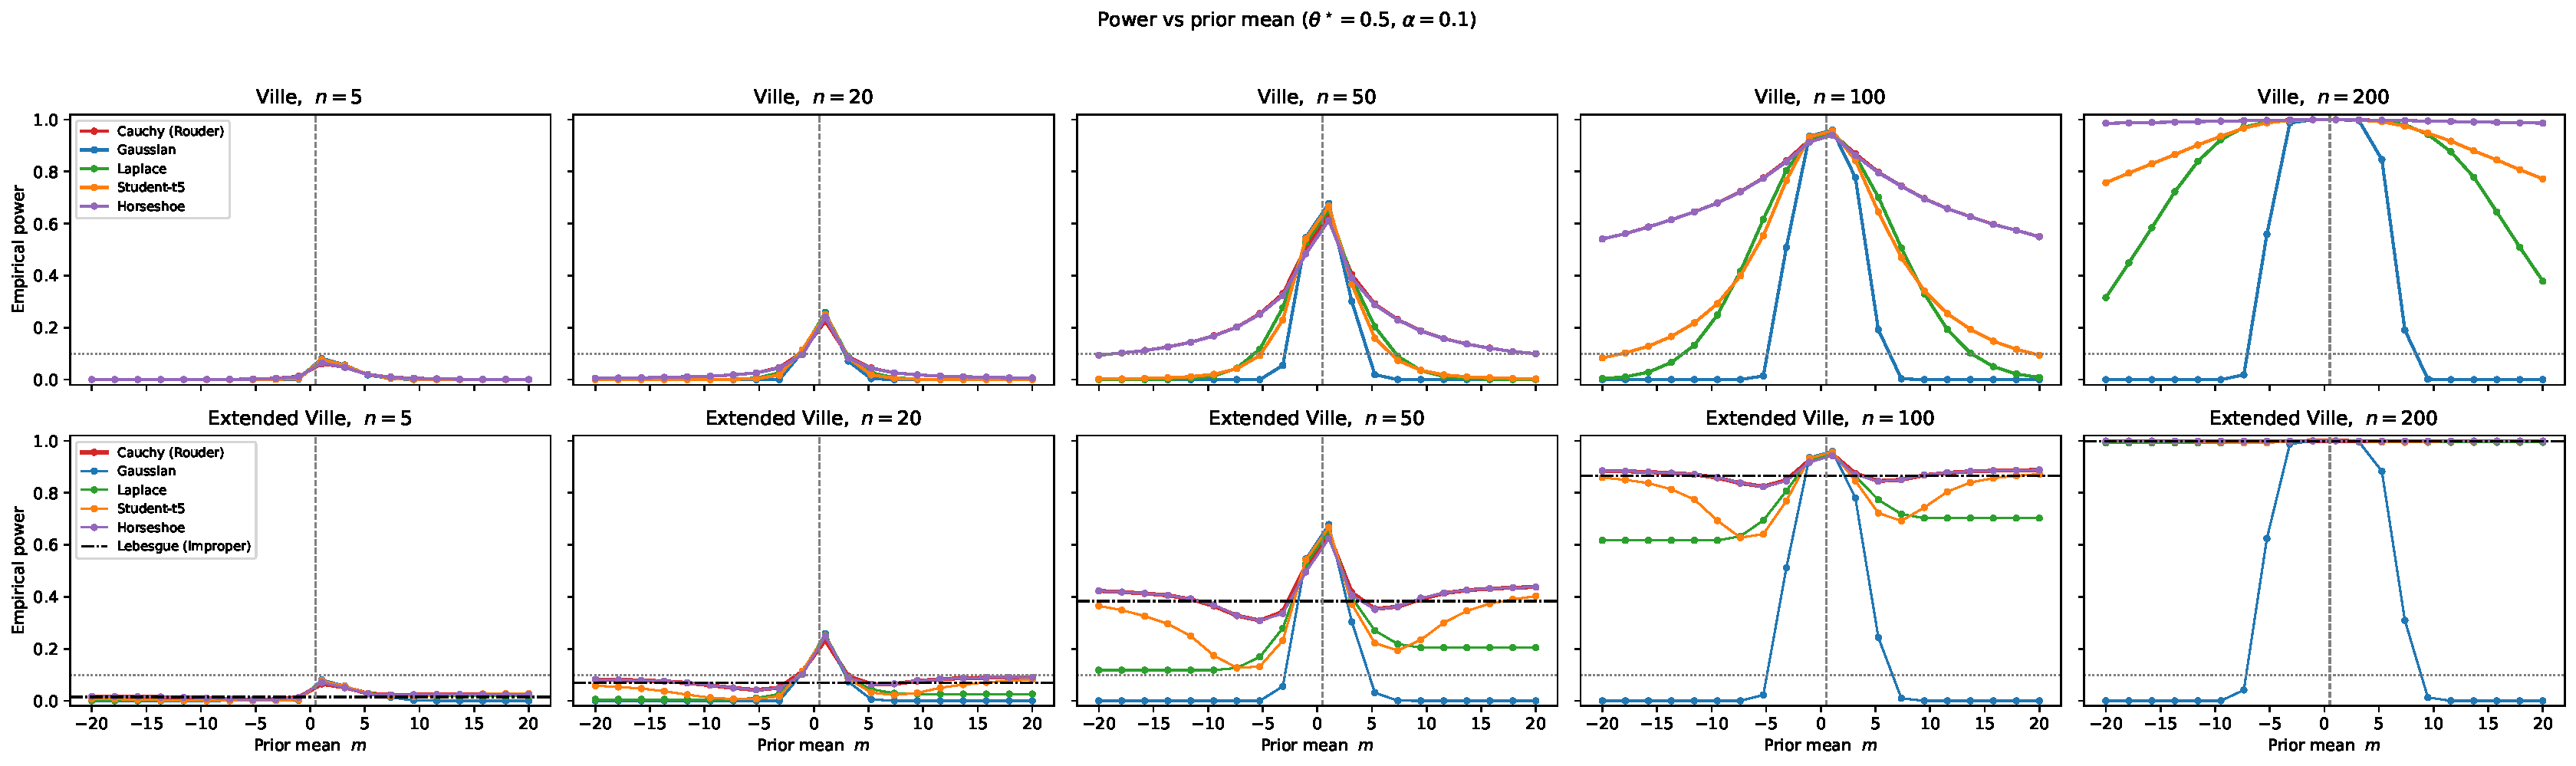
\includegraphics[width=\linewidth]{images/power_vs_m_priors_v2.pdf}
    \caption{Empirical power of the Ville (top row) and extended-Ville
    (bottom row) tests of \(H_0:\theta^\star=0\) under four proper
    priors of unit scale and varying location \(m\), at
    \(\theta^\star=0.5\) and \(\alpha=0.1\), for sample sizes
    \(n\in\{5,20,50,100,200\}\). Each panel uses
    \(B=10{,}000\) data replicates and \(B_{\mathrm{cal}}=100{,}000\)
    calibration replicates. The dashed vertical line marks the
    well-specified location \(m=\theta^\star\); the dotted horizontal
    line marks the level \(\alpha\); the dash-dotted black line in
    the bottom row marks the noninformative Lebesgue extended-Ville
    baseline, which is independent of \(m\)
    by construction. The Cauchy curve (red, thick) reproduces the Rouder--JZS Bayes
    factor of \cite{Rouder2009}.}
    \label{fig:power_vs_m_priors}
\end{figure}

\subsubsection{Running Setup}
We fix the data-generating effect \(\theta^\star=0.5\) and the
significance level \(\alpha=0.1\), and consider sample sizes
\(n\in\{5,20,50,100,200\}\). For each prior shape \(\pi\) of unit scale,
each location \(m\) on a grid
\(\mathcal M=\{-8,-7,\ldots,8\}\), and each pair \((n,m)\), we draw
\(B=10{,}000\) independent datasets
\(Y_{1:n}^{(b)}\stackrel{\mathrm{iid}}{\sim}\mathcal N(\theta^\star,1)\)
and report the empirical Ville and extended-Ville rejection rates
\begin{equation}\label{eq:exp-power}
   \widehat{\mathrm{pow}}_{n,\alpha}^{V}(m)
   = \frac{1}{B}\sum_{b=1}^{B}
     \mathbf 1\!\bigl\{P_{n,0}^{V,\Pi_m}(Y_{1:n}^{(b)})\leq\alpha\bigr\},
   \qquad
   \widehat{\mathrm{pow}}_{n,\alpha}^{eV}(m)
   = \frac{1}{B}\sum_{b=1}^{B}
     \mathbf 1\!\bigl\{P_{n,0}^{eV,\Pi_m}(Y_{1:n}^{(b)})\leq\alpha\bigr\}.
\end{equation}
We compare four proper priors: the Gaussian (G), the Laplace (LP), the
Student-\(t_5\) (T5), and the horseshoe-type density
\(\pi_{\mathrm{HS}}(\theta)=(4\pi)^{-1}\log(1+4/\theta^2)\),
the renormalised Carvalho--Polson--Scott upper bound
\citep{Carvalho2010}, which has the same Cauchy-rate polynomial tail
and soft logarithmic spike at zero as the exact horseshoe and is
computationally more tractable. The Gaussian is the canonical
exponential-square benchmark and falls outside
Assumption~\ref{ass:tails}; the Laplace satisfies Assumption~\ref{ass:tails}
with \(\kappa>0\), \(\beta=0\); and Student-\(t_5\) and the horseshoe
satisfy it with \(\kappa=0\), \(\beta=6\) and \(\beta=2\) respectively.
The improper Lebesgue prior of Section~\ref{ssec:Leb} is included as a
noninformative baseline in the extended-Ville panels; it does not appear
in the Ville panels, since the Ville construction requires a proper prior.

The marginal likelihoods \(M_n^{\Pi_m}\) and the
calibration functions \(g_{0}^{(m)}\) are unavailable in closed form for
the four proper priors and are computed numerically: \(M_n^{\Pi_m}(u_n)\)
by adaptive Gauss--Kronrod quadrature in \(\theta\) on a grid in
\(u_n\in(-\sqrt n,\sqrt n)\) followed by linear interpolation, and the
calibration \(g_{0}^{(m)}\) by Monte Carlo under \(\Prob_0\) with
\(B_{\mathrm{cal}}=100{,}000\) replicates. A single \(\Prob_0\)-sample
of pairs \((Y_1^{(j)},Y_2^{(j)})\) is reused across the entire
\((m,\pi)\) grid by re-evaluating
\(M_2^{\Pi_m}(Y_1^{(j)},Y_2^{(j)})\) at each grid point. The Lebesgue
baseline uses the closed forms of Theorems~\ref{thm:Mn-Leb}
and \ref{thm:gLeb} and incurs no Monte Carlo error in the calibration.


\subsubsection{Interpretation}\label{ssec:exp-interp}

Figure~\ref{fig:power_vs_m_priors} confirms the qualitative picture
predicted by Theorems~\ref{thm:CSVille-divergence} and
\ref{thm:recovery}, and refines it across sample sizes. We observe the following.

\emph{Prior-data agreement.} For every prior and every \(n\), the power
curves attain their maximum at \(m=\theta^\star\), where the prior is
correctly centred. At this location the heavier-tailed priors (T5 and
HS) deliver power comparable to the Gaussian and Laplace priors;
the gain over the noninformative Lebesgue baseline is substantial at
small \(n\) and progressively erodes as \(n\) grows, since the data become more informative.

% \emph{Polynomial-tail priors revert smoothly to the noninformative
% benchmark.} As \(|m-\theta^\star|\) grows, the Student-\(t_5\) and
% horseshoe extended-Ville curves descend monotonically and flatten at
% the dash-dotted Lebesgue line, exactly as predicted by
% Theorem~\ref{thm:recovery}: the procedure loses its informative-prior
% power gain but does not collapse, in contrast to the Ville curves which
% descend to zero. The convergence to the Lebesgue line is slowest under
% the horseshoe (heaviest tails) and fastest under the Student-\(t_5\), in
% agreement with the rate analysis of Section~\ref{sec:robust}.

% \emph{The Gaussian prior loses all power.} The Gaussian density falls
% outside Assumption~\ref{ass:tails}, and Figure~\ref{fig:power_vs_m_priors}
% quantifies the consequence: under arbitrary location misspecification,
% the Gaussian extended-Ville curve drops below the Lebesgue baseline and
% ultimately to zero. The Laplace prior, which satisfies
% Assumption~\ref{ass:tails} only with \(\kappa>0\), shows the intermediate
% behaviour predicted in
% Section~\ref{sec:robust}: it reverts to a strictly positive limit
% above the Lebesgue baseline rather than collapsing, but it does not
% recover the noninformative benchmark exactly.

The contrast between the top and bottom rows of
Figure~\ref{fig:power_vs_m_priors} is the essential message: under the
classical Ville construction every proper prior is fragile, while the
extended-Ville construction with polynomial-tail priors enjoys
informative power gains under prior-data agreement and graceful
reversion to the scale-invariant \(t\)-test under arbitrary
prior-data conflict.


\subsection{Simulation $2$}
The experiments above fix the scale of the prior at one and vary its
location. We now complement them with the dual sweep: the prior is
centred at zero and its scale parameter varies on the \(x\)-axis.
This is the canonical parametrisation of the \cite{Rouder2009} Bayesian \(t\)-test, which places a Cauchy prior \(\mathrm{Cauchy}(0,r)\) on the standardised effect size
\(\theta^\star=\mu/\sigma\). We treat the Rouder test here as a benchmark against which our anytime-valid construction can be compared. From the present perspective, the Rouder Bayes factor is precisely the mixture statistic \(M_n^{\Pi_r}(y_{1:n})\) of \eqref{eq:Mn-zero} with \(\Pi_r=\mathrm{Cauchy}(0,r)\), and the calibrated p-variable
\(g^{(r)}(M_n^{\Pi_r})\) of \eqref{eq:p-from-M} turns it into an anytime-valid p-process under the extended Ville construction. The
present subsection can therefore be read as advertising our procedure as a calibration layer that converts the Rouder--JZS Bayes factor into an anytime-valid, prior-guided \(t\)-test with explicit guarantees under prior-data conflict.

\paragraph{Setup.} We keep the data-generating effect \(\theta^\star=0.5\), the level \(\alpha=0.1\), and the sample sizes \(n\in\{5,20,50,100,200\}\), and draw \(B=10{,}000\) independent datasets per cell. For each prior shape \(\pi\) of zero location and each scale \(r\) on a logarithmic grid \(\mathcal R\subset(0,\infty)\) covering four orders of magnitude, the prior is \(\pi_r(\theta)=r^{-1}\pi(\theta/r)\). The
grid \(\mathcal R\) contains the Rouder default \(r=1\) and brackets it by smaller and larger values so that the limits \(r\downarrow 0\) (near-point alternative at zero) and \(r\uparrow\infty\) (maximally diffuse alternative) are both visible. We compare five proper priors: the Cauchy of \cite{Rouder2009}, the Gaussian, the Laplace, the Student-\(t_5\), and the horseshoe-type density \(\pi_{\mathrm{HS}}(\theta)=(4\pi)^{-1}\log(1+4/\theta^2)\). The
Cauchy and horseshoe priors share the polynomial tail rate \(\beta=2\); the Student-\(t_5\) prior has lighter polynomial tails
(\(\beta=6\)); the Laplace prior has Assumption~\ref{ass:tails} with \(\kappa>0\), \(\beta=0\); and the Gaussian falls outside Assumption~\ref{ass:tails}. The improper Lebesgue prior of Section~\ref{ssec:Leb} provides a noninformative, \(r\)-independent
baseline for the extended-Ville panels. Marginal likelihoods and calibration functions are computed exactly as in Algorithm~\ref{alg:power-vs-m}, with the prior location \(m\) replaced by the prior scale \(r\).


\begin{figure}[ht]
    \centering
    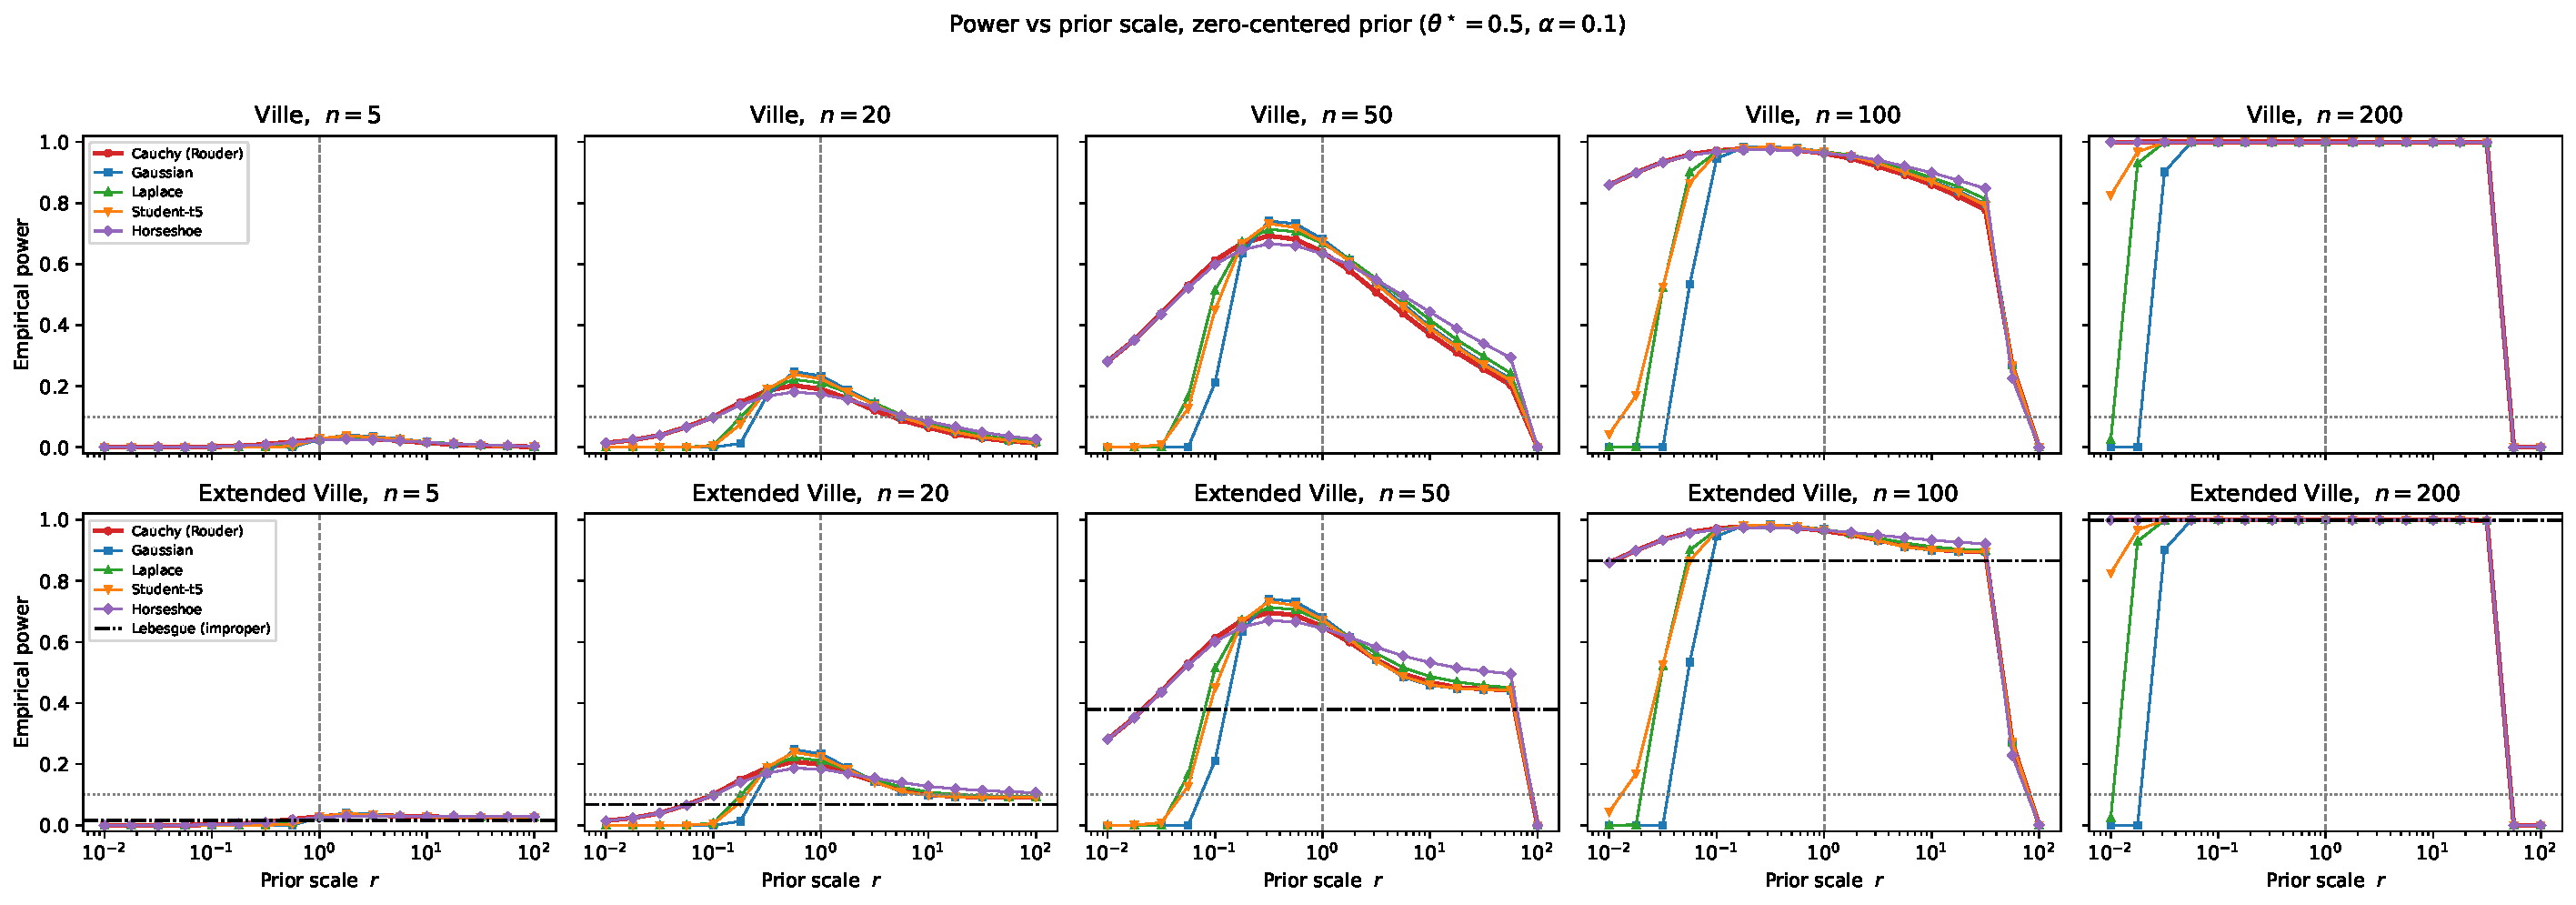
\includegraphics[width=\linewidth]{images/power_vs_r_priors.pdf}
    \caption{Empirical power of the Ville (top row) and extended-Ville
    (bottom row) tests of \(H_0:\theta^\star=0\) under five
    zero-centred proper priors of varying scale \(r\), at
    \(\theta^\star=0.5\) and \(\alpha=0.1\), for sample sizes
    \(n\in\{5,20,50,100,200\}\). The \(x\)-axis is logarithmic in
    \(r\). The dashed vertical line marks the Rouder default \(r=1\);
    the dotted horizontal line marks the level \(\alpha\); the
    dash-dotted black line in the bottom row marks the noninformative
    Lebesgue extended-Ville baseline, which is independent of \(r\).
    The Cauchy curve (red, thick) reproduces the Rouder--JZS Bayes
    factor of \cite{Rouder2009}.}
    \label{fig:power_vs_r_priors}
\end{figure}

\paragraph{Interpretation.}
Figure~\ref{fig:power_vs_r_priors} exhibits three regimes that together complement the location sweep of Figure~\ref{fig:power_vs_m_priors}. 

\emph{Near-point regime, \(r\downarrow 0\).} As the prior contracts onto a point mass at zero, the mixture statistic \(M_n^{\Pi_r}(y_{1:n})\) tends to \(h_{0,n}(y_{1:n})=1\) for every \(y_{1:n}\); both Ville and extended-Ville rejection rates therefore collapse to a level near \(\alpha\) for every prior shape, regardless of the true \(\theta^\star\). At this end of the grid no informative power gain is available, the prior asserts the null, and the heavier-tailed priors are indistinguishable from the lighter ones.

\emph{Moderate scales near \(r=1\).} This is the regime in which the Rouder prior is calibrated to deliver power against effect sizes of order one. All polynomial-tail priors (Cauchy, Student-\(t_5\), horseshoe) attain comparable power here, and the gain over the
Lebesgue baseline is substantial at small \(n\) and progressively erodes as \(n\) grows.

\emph{Diffuse regime, \(r\uparrow\infty\).} For the polynomial-tail priors, the extended-Ville rejection rate approaches the \(r\)-independent Lebesgue baseline (dash-dotted line) as the prior becomes maximally diffuse; the Ville rejection rate, by contrast, descends to zero. The Cauchy curve in the bottom row therefore flattens onto the Lebesgue line at large \(r\), the calibrated
analogue of the well-known fact that the Rouder--JZS Bayes factor with a very wide prior is informationally close to the classical
\(t\)-test \citep[the Jeffreys-Lindley phenomenon, cf.][]{Lindley1957}. The Gaussian and Laplace priors, which fail (respectively, are at the boundary of) Assumption~\ref{ass:tails}, do not enjoy this
reversion. %: the Gaussian curve drops below the Lebesgue baseline and toward zero, and the Laplace curve approaches a strictly positive limit slightly displaced from it.

$\pi_r(\theta) \to \delta_0 (\theta)$ as $r \downarrow 0$, which collapses the mixture statistic to $h_{0,n}(y_{1:n}) = 1$, i.e. the procedure reverts to ``accept $H_0$", rather than to the Lebesgue prior.

For $r \uparrow \infty$, the Lebesgue reversion happens as the prior becomes maximally diffuse, the mixture statistic divided by $\pi(0)/r$ converges to $M_n^{\Leb}$.


\subsection{Real-Data: LLM on Games}
The question that we ask that if GPT-4 doing better or worse than its opponent on average in iterated Prisoner's Dilemma, and how soon can we tell. This can be formulated as a one-sample test of $H_0: \theta^\star = 0$ on per-game payoff differences.

\subsection{Real-Data: NeuroVault}
\cite{bo2024systems} 
Dataset: \url{https://neurovault.org/collections/16266/}




\section{Discussion}\label{sec:discussion}

We have constructed Bayes-assisted anytime-valid \(t\)-tests and
confidence sequences for a Gaussian mean with unknown variance, by
combining the scale-invariant mixture-martingale framework of
\cite{Lai1976} and \cite{Wang2025} with the extended Ville
inequality of \cite{wang2025extended}. The procedure achieves the two
goals identified by \cite{Cortinovis2025} in the known-variance setting: it incorporates prior information for power gains under prior-data agreement, while remaining robust under arbitrary conflict when the prior has polynomial tails.





\bibliography{bayesanytimettest}
\bibliographystyle{alpha}

\end{document} 

